%%%%%%%%%%%%%%%%%%%%%%%%%%%%%%%%%%%%%%%% Klasse Festlegen
\documentclass[Master,BMR,english]{BASE/twbook} 
%\documentclass[Bachelor,BMR,english,fhCitStyle,IEEE]{BASE/twbook} % FH definierte Zitierstandards verwenden 
%%%%%%%%%%%%%%%%%%%%%%%%%%%%%%%%%%%%%%%% Verwendete Packages
\usepackage[utf8]{inputenc} % Zeichen-Enkodierung (evtl. Abweichungen für Apple)
\usepackage[T1]{fontenc}    % Zeichen-Enkodierung
\usepackage{blindtext}      % Platzhaltertexte
\usepackage{minted}         % Darstellung von Code
\usepackage{comment}        % Auskommentieren von ganzen Passagen
\usepackage{csquotes}
\usepackage{algorithm}      % Umgebung f Algorithmen
\usepackage[noend]{algpseudocode}
\usepackage{subcaption}
\usepackage{acronym}
\usepackage{adjustbox}
\usepackage{nameref}
\usepackage{pgfplots}
\usetikzlibrary{positioning,arrows.meta}
\usepackage{import}
\usepackage{multirow}
\usepackage{multicol}
\usepackage{svg}
\usepackage{colortbl} % Paket für Tabellenfarben
%\usepackage[table, x11names]{xcolor} % Für zusätzliche Farboptionen
\providecommand*{\listingautorefname}{Listing}
%\usepackage{cleveref}
                            % Wenn Sie während Ihrer Arbeit
                            % merken, dass Sie zusätzliche Funktionen
                            % benötigen ist hier ein guter Platz um
                            % weitere Packages zu laden
%%%%%%%%%%%%%%%%%%%%%%%%%%%%%%%%%%%%%%%% Querverweisstil zum selbst definieren
\renewcommand{\thefigure}{\arabic{figure}}
%%%%%%%%%%%%%%%%%%%%%%%%%%%%%%%%%%%%%%%% Zitierstil zum selbst definieren
\usepackage[backend=biber, style=ieee]{biblatex}            % LaTeX definierter IEEE- Standard
%\usepackage[backend=biber, style=authoryear]{biblatex}      % LaTeX definierter Harvard-Standard
\addbibresource{Literatur.bib}                              % Literatur-File definieren
%\bibliography{Literatur.bib}
%%%%%%%%%%%%%%%%%%%%%%%%%%%%%%%%%%%%%%%% Einträge für Deckblatt
\title{Robust Rail Track Prediction \\ with Temporal Deep Learning}

\author{Sebastian Goebel, BSc.}
\studentnumber{University of Applied Science: 51912403\and{Luzern University of Applied Sciences and Arts: 23-565-161}}
%\author{Titel Vorname Name, Titel\and{}Titel Vorname Name, Titel}
%\studentnumber{XXXXXXXXXXXXXXX\and{}XXXXXXXXXXXXXXX}

\supervisor{Prof. Dr. Björn Jensen}
%\supervisor[Begutachter]{Titel Vorname Name, Titel}
%\supervisor[Begutachterin]{Titel Vorname Name, Titel}
%\secondsupervisor{Titel Vorname Name, Titel}
%\secondsupervisor[Begutachter]{Titel Vorname Name, Titel}
%\secondsupervisor[Begutachterinnen]{Titel Vorname Name, Titel}

\place{Vienna}
%%%%%%%%%%%%%%%%%%%%%%%%%%%%%%%%%%%%%%%% Danksagung/Kurzfassung/Schlagworte
\kurzfassung{\blindtext}
\schlagworte{Schlagwort1, Schlagwort2, Schlagwort3, Schlagwort4}
\outline{\blindtext}
\keywords{Keyword1, Keyword2, Keyword3, Keyword4}
\acknowledgements{\blindtext}
\setListingsAndAcronyms % Definition der Namen für Quellcodeverzeichnis 
%%%%%%%%%%%%%%%%%%%%%%%%%%%%%%%%%%%%%%%% Ende des Headers
%%%%%%%%%%%%%%%%%%%%%%%%%%%%%%%%%%%%%%%% Beginn des Dokuments
\begin{document}
%%%%%%%%%%%%%%%%%%%%%%%%%%%%%%%%%%%%%%%% 
\maketitle
%%%%%%%%%%%%%%%%%%%%%%%%%%%%%%%%%%%%%%%% Beginn des Inhalts
%%%%%%%%%%%%%%%%%%%%%%%%%% Introduction %%%%%%%%%%%%%%%%%%%%%%%%%%

% Include the first subsection from an external file
\chapter{Introduction}
Etwas Text... Hier kommen noch einige Abkürzunge vor zum Beispiel \ac{ABC},\ac{WWW} und \ac{ROFL}.

\begin{itemize}
    \item Worum geht es?
    \item Was mach ich und warum?
    \item Motivation
    \item Problem
    \item Ziel
\end{itemize}

Autonomous vehicles are increasingly considered a groundbreaking technology of the future. \cite{FraunhoferInstituteforCognitiveSystemsIKS.21.10.2024}

\section{Erste Überschrift Tiefe 2 (section)}
blindtext

\subsection{Erste Überschrift Tiefe 3 (subsection)}
blindtext

\subsubsection{Erste Überschrift Tiefe 4 (subsubsection)}
blindtext
\cite{orf2024toetlicherZugunfall}

%%%%%%%%%%%%%%%%%%%%%%%%%%%%%%%%%%%%%%%%%%%%%%%%%%%%%%%%%%%%%%%%%%
%%%%%%%%%%%%%%%%%%%%%%%% State of the Art %%%%%%%%%%%%%%%%%%%%%%%%
\clearpage                                                       % Beginne neue Seite

% Include the first subsection from an external file
\chapter{State of the Art}
\label{sec:stateOfTheArt}

To get an idea of possible solutions and the most promising approaches, this chapter summarizes the most relevant state-of-the-art.
This chapter includes general information and task-specific projects focusing on the rail domain.
In \autoref{sec:networkArchitectures} describes the most relevant developments in network architectures.
Then, an introduction to different vision tasks and their approaches is given to serve as an overview in \autoref{sec:differentApproaches}.
Because three of those different vision tasks are relevant to this work, they are described in more detail.
\autoref{sec:ObjectDetection} depicts real-time object detectors, \autoref{sec:SemanticSegmentation} describes semantic segmentation approaches, and \autoref{sec:lineDetection} describes other approaches, which are summarized as line detection approaches.
\autoref{sec:transformerBasedApproaches} describes transformer-based approaches for object detection and segmentation tasks.
At one point in this work, \cite{tepNet2024} is selected as a baseline for further experiments.
Therefore, this project is explained in more detail in \autoref{sec:baselinepaper}.
Temporal model architectures are described in \autoref{sec:temporalModelArchitecture}.
\autoref{sec:datasets} thoroughly describes available datasets for the rail domain.

%%%%%%%%%%%%%%%%%%%%% network architectures %%%%%%%%%%%%%%%%%%%%%

\section{Network architectures}
\label{sec:networkArchitectures}

One of the first CNN architectures was the \textbf{Le-Net5} \cite{LeNet5}.
This CNN was proposed to classify handwritten digits.
It used 5 convolution and pooling layers.
14 years later CNNs were rediscovered with the introduction of \textbf{AlexNet} <Quelle: AlexNet> in 2012.
In the \ac{ILSVRC} <Quelle> in 2012 \textbf{AlexNet} outperformed traditional algorithms and showed the potential of CNNs.
Consequently, it is often considered the starting point of the CNN era in the literature.
Since then research has shown a rapid development of CNN architectures, consistently striving for greater accuracy or speed \cite{networkArchitectureSurvey}.

\vspace{1cm} % Größerer Abstand zwischen den Reihen

\noindent Several major advancements up to now include:

\begin{itemize}
    \item In 2014 two popular architectures were introduced, which still are often used for state-of-the-art comparisons. Firstly, the \textbf{\ac{VGGNet}} \cite{VGGNet2015} used small three-by-three filters and many layers providing a deep network architecture. Secondly, the \textbf{Inception} network or \textbf{GoogLeNet} \cite{InceptionNet}. To extract features in a range of various scales, this architecture utilized different filter sizes.
    \item In 2015 the \textbf{ResNet} architecture \cite{ResNet} introduced the concept of residual learning with shortcut connections. By skipping layers, this framework enabled the training of deeper networks with over a hundred layers.
    \item In 2016 \textbf{DenseNets} \cite{DenseNets} was introduced to further deal with the problem of vanishing gradients. This architecture implemented a connection between each layer and every following layer ensuring maximum information flow.
    \item In 2017 \textbf{MobileNets} \cite{MobileNetV1} \cite{MobileNetV2} \cite{MobileNetV2Arxiv} \cite{MobileNetV3} was developed for applications in mobile devices. Since hardware with limited capabilities is used, the main focus of MobileNet architectures lies on efficiency. The utilization of depthwise separable convolutions allowed small model sizes and fast latencies.
    \item In 2019 \textbf{EfficientNets} \cite{EfficientNet} was introduced to further explore greater trade-offs between accuracy and efficiency, by using scaling methods for model architectures. 
\end{itemize}

\subsection{ResNets}

https://medium.com/@cpt1995daas/evolution-of-convolutional-neural-network-cnn-architectures-44f2109268a1

blindtext

\subsection{DenseNets}

blindtext

\subsection{MobileNetV3}

blindtext

\subsection{EfficientNets}

blindtext



%%%%%%%%%%%%%%%%%%%%%%%%%%%%%%%%%%%%%%%%%%%%%%%%%%%%%%%%%%%%%%%%%%

%%%%%%%%%%%%%%%%%%%%% Different approaches of vision tasks %%%%%%%%%%%%%%%%%%%%%
\clearpage
\section{Different approaches of vision tasks}
\label{sec:differentApproaches}

Many different kinds of vision tasks input image data.
These use cases outline broad guidelines for designing neural network architectures and the workflow of such a model by which the desired output is produced.
\autoref{fig:differentApproaches} shows the outputs of the most commonly used strategies in the literature that might be relevant for rail track prediction or a part of it.
The input image for all models is visualized in \autoref{fig:differentApproaches_classification} without the added text in the top right corner.

\vspace{1cm} % Größerer Abstand zwischen den Reihen

\begin{figure}[H]
    \centering
    
    % Erste Reihe
    \begin{subfigure}{0.328\textwidth}
        \includegraphics[width=\linewidth]{PICs/differentApproaches/classification_v2.jpg}
        \caption{classification}
        \label{fig:differentApproaches_classification}
    \end{subfigure}
    \hfill
    \begin{subfigure}{0.328\textwidth}
        \includegraphics[width=\linewidth]{PICs/differentApproaches/object_detection.jpg}
        \caption{object detection}
        \label{fig:differentApproaches_object_detection}
    \end{subfigure}
    \hfill
    \begin{subfigure}{0.328\textwidth}
        \includegraphics[width=\linewidth]{PICs/differentApproaches/instance_segmentation_v2.jpg}
        \caption{instance segmentation}
        \label{fig:differentApproaches_instance_segmentation}
    \end{subfigure}

    \vspace{0.1cm} % Größerer Abstand zwischen den Reihen

    % Zweite Reihe
    \begin{subfigure}{0.328\textwidth}
        \includegraphics[width=\linewidth]{PICs/differentApproaches/semantic_segmentation.jpg}
        \caption{semantic segmentation}
        \label{fig:differentApproaches_semantic_segmentation}
    \end{subfigure}
    \hfill
    \begin{subfigure}{0.328\textwidth}
        \includegraphics[width=\linewidth]{PICs/differentApproaches/panoptic_segmentation.jpg}
        \caption{panoptic segmentation}
        \label{fig:differentApproaches_panoptic_segmentation}
    \end{subfigure}
    \hfill
    \begin{subfigure}{0.328\textwidth}
        \includegraphics[width=\linewidth]{PICs/differentApproaches/line_detection.jpg}
        \caption{line detection}
        \label{fig:differentApproaches_line_detection}
    \end{subfigure}

    \caption{The most common applications in vision tasks that are supported by neural networks. Shown are \ac{GT} examples for each usage domain. The input image is visualized in (a) without the added text in the top right corner \cite{panopticsegmentation2019}.}
    \label{fig:differentApproaches}
\end{figure}

\clearpage
\noindent\textbf{Classification} describes the scene in the input image with only one label.
\autoref{fig:differentApproaches_classification} shows a possible example with the label added in the top right corner of the input image.
No further information is available from the output of a classification method.

\vspace{1cm} % Größerer Abstand zwischen den Reihen

\noindent\textbf{Object detection} combines classification with localization.
This technique outputs so-called bounding boxes that also include positional information of objects.
Additionally, class labels are assigned to each bounding box which show what has been recognized.

\vspace{1cm} % Größerer Abstand zwischen den Reihen

\noindent\textbf{Instance segmentation} expands on object detection by not just outputting bounding boxes.
It generates binary masks within each bounding box, enabling more accurate identification of the pixels that belong to the object and those that do not.
Regions within the bounding box that are not part of the object are disregarded.

\vspace{1cm} % Größerer Abstand zwischen den Reihen

\noindent\textbf{Semantic segmentation} is a method that outputs a class label for each pixel of the input image.
Consequently, the output consists of a mask with the same width and height as the input image.
An example is shown in \autoref{fig:differentApproaches_semantic_segmentation} with people and cars being two of the output labels.
In this work, semantic segmentation can be used for filtering out the rail track for example.

\vspace{1cm} % Größerer Abstand zwischen den Reihen

\noindent\textbf{Panoptic segmentaiton} combines semantic segmentation and instance segmentaiton.
It makes the difference between so-called "things" and "stuff" \cite{panopticsegmentation2019}.
Examples of "things" in \autoref{fig:differentApproaches_panoptic_segmentation} are countable objects like cars and people.
Examples of "stuff" are the road, buildings or the sky.
As with semantic segmentation, this method outputs a pixel-wise classification.
This mask also has the same dimensions as the input image.
However, while semantic segmentation assigns the same class to different instances of the same objects, panoptic segmentation can differentiate between different "things".
\autoref{fig:differentApproaches_panoptic_segmentation} shows that each car or person has its unique class label.

\vspace{1cm} % Größerer Abstand zwischen den Reihen

\noindent\textbf{Line detection} algorithms are usually tailored to filter out lines like road markings or rails.
\autoref{fig:differentApproaches_line_detection} shows a possible output in the road domain of such an algorithm.
Even though in the field of line detection a lot of work has been done in the road domain, the main focus of this work is on applications in the rail domain.
Furthermore, many state-of-the-art papers include outputs in the form of binary masks with the same dimensions as the input image.
While these models solve the line detection problem, they use pixel-wise classification and technically fall into the category of semantic segmentation.
In this work, these papers are therefore reviewed in the corresponding section.
Solely techniques not based on semantic segmentation are included in the line detection section.

\clearpage

\noindent Following a brief description of all the various approaches, it becomes clear that only object detection, semantic segmentation, and line detection are viable options for rail track prediction.
Object detection can be used to filter out switches in the image and their states.
The information if a switch state is left or right can be useful for predicting the leading rail in an application.
Semantic segmentation can be used to identify the track itself on the pixel level.
This solution provides a more intuitive solution for train operators where not only a state is outputted, but the track is visualized in the image.
Ideally, object detection and track segmentation are combined so that only the train's track is displayed.
The third approach, which must not be overlooked are line detection algorithms.
While the output and techniques slightly differ from semantic segmentation, they also provide important pixel-wise information about the track.
As the other approaches are not suitable or relevant for this use case, they are excluded. The next few sections focus on the three techniques mentioned and describe them in more detail.

%%%%%%%%%%%%%%%%%%%%%%%%%%%%%%%%%%%%%%%%%%%%%%%%%%%%%%%%%%%%%%%%%%

%%%%%%%%%%%%%%%%%%%%% Object Detection %%%%%%%%%%%%%%%%%%%%%

\section{Real-time Object detection (2 Seiten)}
\label{sec:ObjectDetection}

In 2012 <Quelle: ImageNet Classification with Deep Convolutional Neural Networks> showed that deep convolutional networks are capable of extracting abstract feature representations from images in a robust manner.
Enabling accurate classification.
In 2014 <Quelle: Rich Feature Hierarchies for Accurate Object Detection and Semantic Segmentation> introduced Regions with CNN features (RCNN).
Since then the development of CNNs can be grouped into two different detection techniques: "two-stage detectors" and "one-stage detectors".

\subsection{Two-stage detectors}

Two-stage detectors usually follow a "coarse-to-fine" process, which firstly includes a region proposal and secondly a classification and a refinement of regions.
Well-known examples are the R-CNN, Fast R-CNN, Faster R-CNN, Mask R-CNN, and FPN <Quellen>.
Even though these models achieve promising accuracy results, they are highly complex, which increases inference time.
Consequently, two-stage detectors are usually unsuitable for real-time-critical applications.
Since all of the use cases of the implementation of this work involve real-time capable applications, the inference time is of great importance.
Therefore two-stage detectors are not further considered for this work.

\subsection{One-stage detectors}

Single-stage detectors or one-stage-detectors combine the classification and localization in one step making them fast enough for real-time applications.
The first single shot detector was the You Only Look Once (YOLO) <Quelle: YOLO1>, which operates with up to 155 FPS.
Yolo is the first approach, which reframed the object detection task as a regression problem.
The introduced model consists of a single neuronal network, allowing end-to-end training.
This model first divides the image into a grid and then simultaneously predicts bounding boxes and the probabilities of classes.
Proving to be a fast object detector, <Quelle: YOLO v1> presented the beginning of a whole series of real-time capable models.
Since, <Quelle: YOLO v1> still shows decreased accuracy in the localization of small objects, versions YOLOv3, YOLOv4, YOLO9000, and SSD particularly focused on this issue.
However, YOLOv7 and YOLOv9 are among the latest real-time object detection models, emphasizing both high speed and improved parameter utilization.

\subsubsection{YOLO v7}
\label{subsubsec: YOLO v7}

The YOLO v7 introduced in 2022 is a subsequent work from the YOLO v4.
It surpasses most object detectors in both accuracy and speed, with inferences from 5 FPS to 160 FPS.
The main contributions of YOLOv7 are several methods that increase the accuracy without decelerating inference.
To achieve that it incorporates a planned re-parameterized strategy, which can be utilized for layers in various models.
Furthermore, YOLO v7 also uses new label assignment methods called "coarse-to-fine lead head guided label assignment".
Additionally, extend and compound scaling techniques are used.
The introduced methods not only increased speed and accuracy, but also decreased the number of parameters of the model by about 40\%.
This presents an advantage for this work since the final system is supposed to operate on an embedded device.

\subsubsection{YOLO v9}
\label{subsubsec:YOLOv9}

The YOLOv9 is yet another follow-up work from YOLOv7.
Released in February 2024, it is the most recent model in the YOLO series.
<Quelle> states that most models lose information through spatial transformations and layer-by-layer feature extraction.
Therefore, the YOLO v9 model focuses on reversible functions and information bottlenecks.
Consequently, the main contributions of <Quelle: yolov9> are a Programmable Gradient Information (PGI) concept, which utilizes auxiliary reversible branches, and a Generalized Efficient Layer Aggregation Network (GELAN), which further increases the usage of existing parameters.
The proposed models prove to be lightweight while still being accurate and fast, outperforming current real-time object detection models.
The characteristics of these models indicate that they are also applicable to this work.


%%%%%%%%%%%%%%%%%%%%%%%%%%%%%%%%%%%%%%%%%%%%%%%%%%%%%%%%%%%%%%%%%%

%%%%%%%%%%%%%%%%%%%%% Semantic Segmentation %%%%%%%%%%%%%%%%%%%%%

\clearpage 
\section{Semantic Segmentation}
\label{sec:SemanticSegmentation}

The first approach to filter out the rail tracks in front of the train was proposed by <Quelle: 2018: Efficient Rail Area Detection Using Convolutional Neural Network [in TEP]> in 2018.
A SegNet <Quelle: SegNet> inspired network for semantic segmentation is extended with mixed pooling <Quelle> and atrous spatial pyramid pooling (ASPP) from DeepLab.
After the proposed semantic segmentation network outputs a binary mask with pixel labels being track or no track, a polygon fitting technique is utilized to refine the tracks further.

In 2019 <RailNet: A Segmentation Network for Railroad Detection> introduced the RailNet architecture.
This model uses a ResNet-50 <Quelle ResNet> backbone and a fully convolutional network <Quelle in TEP-Net> to segment the rail tracks.
The network is designed in a pyramid structure <Quelle: 2017 Feature pyramid networks for object detection>, in which features of every ResNet stage are summed and up-sampled.
This combines low and high-level features, resulting in an enhanced performance.
<Quelle: RailNet: A Segmentation Network for Railroad Detection> reports higher accuracy than state-of-the-art segmentation models at the time with speeds up to 20 FPS.
Tests are made on the introduced RSDS dataset further described in <Dataset section>.

In 2019 RailSem19 <Quelle: RailSem19> introduced the first publicly available dataset for the rail domain.
This dataset also includes annotations for semantic segmentation tasks and experimented with a FRRNB model <Quelle: Full-Resolution Residual Networks for Semantic Segmentation in Street Scenes>.
This dataset is widely used in the community when working in the rail domain.

<Quelle: 2020 RailNet: An Information Aggregation Network for Rail Track Segmentation> already uses a subset of RailSem19 in 2020.
Another RailNet model is proposed that uses a VGG16 backbone and an Information Aggregation Module.
<Quelle: 2020 RailNet: An Information Aggregation Network for Rail Track Segmentation> only predicts the rails in RailSem19, other annotations are ignored.
The characteristics of rails like placement and structure are considered.
Therefore the integrated module is implemented to improve spatial relationship between features on both the vertical and horizontal axes.

<Quelle: 2022 Automated Semantic Segmentation for Autonomous Railway Vehicles> also used RailSem19.
The U-Net <Quelle: U-Net> architecture is trained on four different subsets of RailSem19, including 2, 3, 4, or all 19 classes.
Additionally, A cropping method is implemented to account for the difference in resolutions between the recommended one for U-Net and one of RailSem19's images.

<Quelle: 2022 Application of Rail Segmentation in the Monitoring of Autonomous Train’s Frontal Environment> used the RailSet dataset <Quelle: 2022 RailSet: A Unique Dataset for Railway Anomaly Detection>, which is an extension of RailSem19 for segmentation and anomaly detection tasks.
For details of the RailSet dataset please refer to <dataset section>.
<Quelle: 2022 Application of Rail Segmentation in the Monitoring of Autonomous Train’s Frontal Environment> trained U-Net <Quelle: U-Net> and FRNN <Quelle: FRNN> and incorporated horizontal flips and zooming into the data augmentation.

In 2020 <Quelle: Railroad semantic segmentation on high-resolution images> proposed a U-Net-inspired <Quelle: U-Net> semantic segmentation network.
It combines a ResNet-34 backbone and includes connections to the upsampling blocks.
At the deepest level, a spatial pyramid pooling (SPP) <Quelle: Spatial pyramid pooling in deep convolutional networks for visual recognition> and on the skip connections squeeze-and-excitation blocks <Quelle: wie bei mobilenet> are used.
Tests on RailSem19 <Quelle: RailSem19>, show that it outperforms <Quelle: 2019 RailNet: A Segmentation Network for Railroad Detection> in accuracy with a speed of 20 FPS.
Additionally, <Quelle: Railroad semantic segmentation on high-resolution images> introduced the concept of "possible tracks", which are all paths the train could follow under the assumption that the state of switches cannot be determined.
For this, a rule-based post-processing algorithm is proposed. <Figure xy> shows the concept of possible paths.

\vspace{1cm}

<vielleicht figure possible tracks von Quelle: Railroad semantic segmentation on high-resolution images>

\vspace{1cm}

In 2023 <Quelle: TPE-Net: Track Point Extraction and Association Network for Rail Path Proposal Generation> further investigated the task of possible tracks and introduced Track Point Extraction and Association Network (TPE-Net).
It consists of a DenseNet-inspired architecture, which is trained and tested on RailSem19 and outputs regressed heatmaps besides the segmented rails.
An example of such a heatmap is an image with one channel that shows the probability of each pixel being within a rail track.
The segmentation mask and the heatmaps are then used by a complex post-processing approach.
This process includes track point clustering, the creation of track segments, and the creation of a path tree, which is then used to generate all possible tracks.
Refinement is done by removing redundant paths and polynomial fitting.
Because of the complexity of this system, <Quelle: TPE-Net: Track Point Extraction and Association Network for Rail Path Proposal Generation> reports speeds up to 12 FPS making this system unsuitable for real-time applications.
Additionally, it is stated that problems arise when switches are present.

In 2022 <Quelle: RailVID: A Dataset for Rail Environment Semantic> proposed the RailVID dataset, which consists of infrared images instead of RGB data to improve the system's abilities in challenging situations such as the absence of ambient light.
The dataset is described in <Dataset section> in more detail.
After collecting data, <Quelle: RailVID: A Dataset for Rail Environment Semantic> experimented with widely used CNNs for semantic segmentations, like CGNet <Quelle>, DeepLabv3+ <Quelle>, and BiSeNet <Quelle>.
Additionally, an improved BiSeNet architecture is proposed with consideration of the infrared data. Performance is enhanced by added layers to fuse low-level features.

In 2021 <Accurate and Lightweight RailNet for Real-Time Rail Line Detection> proposed another architecture called RailNet.
It consists of an Encoder-Decoder structure incorporating depth-wise convolutions and a Segmentation Soul block, inspired by the context embedding block of BiSeNetV2 <Quelle: BiSeNetV2>.
Additionally, a port processing algorithm is utilized that is based on sliding window detection.
<Accurate and Lightweight RailNet for Real-Time Rail Line Detection> reports speeds up to 74 FPS proving that this system is real-time capable.

A topic that could be interesting is anomaly detection because many state-of-the-art approaches use semantic segmentation as a preprocessing step.
<2021 Near Real-time Situation Awareness and Anomaly Detection for Complex Railway Environment> utilizes a BiSeNet architecture for segmenting rails, which is tailored for the anomaly detection task.
This network can detect small objects on the track.
Therefore accuracy is preferred over speed, resulting in a system that is not real-time capable.

\subsection{Example Überschrift}

blindtext

\subsection{Example Überschrift}

blindtext hallo

%%%%%%%%%%%%%%%%%%%%%%%%%%%%%%%%%%%%%%%%%%%%%%%%%%%%%%%%%%%%%%%%%%

%%%%%%%%%%%%%%%%%%%%% Transformer based appraoches %%%%%%%%%%%%%%%%%%%%%

\section{Transformer-based appraoches}
\label{sec:transformerBasedApproaches}

In recent years, other research fields have arisen.
Visual grounding tasks, for example, input text descriptions and try to localize the described objects in a scene \cite{openvocabularysurvey2024}.
Visual grounding can deal with semantic segmentation or bounding boxes.
One of the most promising approaches is Grounding DINO \cite{groundingdino2024}, which combines grounding and transformer-based detection in a single framework, achieving strong results in object detection benchmarks.
This framework cannot be used for segmentation tasks \cite{glipv22022}.
Grounding DINO achieves a speed of 8.37 FPS, which makes it too slow for real-time applications \cite{groundingdino2024}.
The model is trained on 64 NVIDIA A100 GPUs, far exceeding the resources available for this work.
Despite a strong performance in object detection benchmarks, there are several reasons why this model is not further considered.
This model is too slow for real-time applications; there is a lack of data to leverage this model's advantages fully, and it would not make sense to consider it for use on limited embedded devices.

\vspace{0.5cm}

Another concept is open vocabulary detection, which extends the number of classes labeled and used during training (base classes).
The goal is also to predict novel classes during inference \cite{openvocabularysurvey2024}.
One common approach to enabling the open vocabulary setting for close-set detectors is changing the fixed classifier weights to text embeddings derived from a visual language (VLM) model as visually represented in \autoref{fig:openvocabulary} \cite{openvocabularysurvey2024}.
In this context, close-set detectors are traditional detectors that only work with base classes \cite{anonymous2024openvocabulary}.

\begin{figure}[H]
    \centering
    \includegraphics[width=0.55\linewidth]{PICs/tansformerSOTA/openvocabulary.jpg}
    \caption{A common structure of open vocabulary models for object detection and semantic segmentation. Vision part predicts class embeddings and VLM-text part (CLIP or ALIGN) generates class embeddings. They are compared with a dot product and the one with the highest score is the output. \cite{openvocabularysurvey2024}.}
    \label{fig:openvocabulary}
\end{figure}

The GLIP series \cite{GLIPv12022} \cite{glipv22022} are examples of such open vocabulary methods.
GLIPv2 uses a Swin Transformer \cite{swinTransformer2021} as an encoder and other transformers for text encoding.
While grounding DINO solely supports object detection tasks, GLIPv2 can be used for segmentation tasks \cite{groundingdino2024}.
The model allows object detection, instance segmentation and can perform Vision-Language understanding tasks \cite{glipv22022}.
GLIPv2 achieves comparable performance to the state-of-the-art in localization tasks.
However, inference speeds only reach up to 4.12 FPS in object detection on an NVIDIA V100.

\vspace{0.5cm}

Another intresting approach is introduced in Segment Anything \cite{segmentAnything2023} and aims to build a universal segmentation model.
Consequently, this model is trained on a dataset with over one billion masks on 11 million images.
Segment Anything \cite{segmentAnything2023} allows zero-shot detection, meaning the model can segment classes not included in training \cite{segmentAnything2023} \cite{openvocabularysurvey2024}.
\cite{segmentAnythingOnline} provides an interface to interact with this model.
Segment Anything accepts an image as an input.
The model can then segment the region of interest, which the user defines with anchor points.
\cite{segmentAnything2023} includes a prompt encoder in the model to allow such flexible prompts.
Other modules included are an image encoder, a mask decoder, and an image embedding module.
This work does not include any types of prompts in the input data.
Therefore, this model is not considered further despite achieving impressive results in segmentation tasks.
The successor model, Segment Anything 2 \cite{segmentAnything22024}, is published while finalizing this work, which solves a similar task but accepts video material as input.
The model allows object tracking in videos.
A brief experiment is conducted, applying a pre-trained SAM2 model on a rail domain video and described in the \autoref{sec:discussion} because further research is out of the scope of this work.

Table 1 in \cite{openvocabularysurvey2024} gives a detailed overview of state-of-the-art open vocabulary detection and segmentation approaches.
(hier vielleicht it includes state-of-the-art approaches like [und dann eine aufzählung]).
It lists the text models and vision models used by an approach.
Text models include CLIP \cite{CLIP2021}, BERT \cite{BERT2019}, or ALIGN \cite{ALIGN2021}, among others.
This work does not include text information in the input data, as the goal is to develop a rail track prediction system that solely bases predictions on image data.
Therefore, text models are not utilized.
The relevant parts of state-of-the-art open vocabulary approaches are the vision models.
These either consist of network architectures like Faster R-CNN or EfficientNet \cite{openvocabularysurvey2024}, which are already described in \autoref{sec:ObjectDetection} and \autoref{sec:networkArchitectures}.
Other vision models are transformer-based, like Swin Transformer \cite{swinTransformer2021}, CLIP-vision \cite{CLIP2021}, ViT \cite{ViT2021}, MaskFormer \cite{MaskFormer2021}, Mask2Former \cite{mask2Former2022}, and DINO \cite{DINO2022}.
Also commonly used MaskFormer and Mask2Former, only reach 17.6 FPS and 8.6 FPS on an NVIDIA V100 GPU \cite{mask2Former2022}.

While these open-vocabulary or universal models usually present promising approaches in terms of accuracy, most of them are transformer-based approaches and suffer from a low frame rate (below 30 FPS) \cite{carion2020endtoendobjectdetectiontransformers, groundingdino2024, swinTransformer2021, MaskFormer2021, mask2Former2022, glipv22022} making them unsuitable for real-time applications.
Therefore, they are not considered further in this work.
An additional issue is that large amounts of computing resources are often needed to train transformer-based models, which exceeds the resources of this work \cite{groundingdino2024} \cite{glipv22022}.
Also, in inference, a strong GPU is usually utilized \cite{groundingdino2024} \cite{glipv22022}.
Since the goal of this work is to be capable of real-time operation on limited embedded hardware, lightweight models are preferred.
Therefore, transformer-based models are not considered for further research.

%%%%%%%%%%%%%%%%%%%%%%%%%%%%%%%%%%%%%%%%%%%%%%%%%%%%%%%%%%%%%%%%%%

%%%%%%%%%%%%%%%%%%%%% Line Detection %%%%%%%%%%%%%%%%%%%%%

\clearpage                                                       % Beginne neue Seite
\section{Line Detection}
\label{sec:lineDetection}

Many line detection algorithms stem from the road domain, to detect lanes.
This is done for autonomous or safety systems for cars.
Most algorithms are trained on datasets like TuSimple \cite{tuSimpleDataset} or CULane \cite{cuLaneDataset}, which include images taken in the front view of cars.
While TuSimple is captured on US highways CULane's images are from Beijing.
<Figure xy> shows examples of TuSimple.

\vspace{1cm}

Bild: $https://github.com/TuSimple/tusimple-benchmark/blob/master/doc/lane_detection/assets/examples/lane_example.jpg$

\vspace{1cm}

\cite{LaneDetectionCascadedCNNs2019} proposed one of the first lane detection approaches on TuSimple.
The proposed method detects lanes and classifies the kind of lane.
Two cascaded CNNs are utilized, the first one is an encoder-decoder network for instance segmentation and the second one is a classification network.

However encoder-decoder structures are very similar to the techniques used for semantic segmentation.
Other structures for lane detection include key point extraction, grid systems, or polyline regression.

Keypoint detection on the road

\cite{LineCNN2020} proposed Line-CNN, which includes a ResNet backbone and an introduced Line Proposal Unit.
The model suggests a series of lines to locate road lanes.
After the proposal, the line with the highest confidence score is fitted with horizontal offsets to match the actual lane.

\cite{CurveLaneNAS2020} proposed a network, that predicts road lanes with the horizontal offsets from a pre-defined vertical anchor.
Additionally, \cite{CurveLaneNAS2020} utilized a \ac{NAS} to find the optimal architecture for this task.

Similar to Line-CNN, the method proposed in \cite{KeepEyesOnLane2021} also proposes lines with confidence scores and fits the resulting output with horizontal offsets.
The novelty of this approach is in an introduced attention mechanism based on anchors.
This added module results in higher accuracy and a much faster model with speeds up to 250 \ac{FPS}.

Another approach that uses key points is introduced in \cite{GANet2022}.
This architecture utilizes a Lane-aware Feature Aggregation module to strengthen the connection between neighboring key points and archives state-of-the-art performance.

Grid system

An approach that uses grid systems is proposed by \cite{laneDetectionGrid2020}.
Here a row-wise classification is done for a predefined number of grids.
The number of grids is equivalent to the number of lanes that can be detected.

polyline regression

A regression approach is proposed in \cite{PolyLaneNetRoad2021}, that predicts the polynomials of lanes.
ResNet and EfficientNet backbones are used to extract features, that are then used to forecast lines.
Each line includes the coefficients of a polynomial, a starting parameter, and a confidence score.
Additionally, a shared horizon line is predicted, where all polylines end.
Compared to other state-of-the-art approaches, \cite{PolyLaneNetRoad2021} proposes a computationally efficient method with speeds up to 115 \ac{FPS}.
While accuracy is lower than with other methods, it still is comparable.

\cite{DetectingLanesWithBezierCurves2023} proposed an approach that predicts the parameters of a cubic Bezier curve.
This curve is fitted in the area defined by four control points.
A typical backbone like ResNet with additional feature flip fusion modules is utilized.
After a pooling and two convolutional layers, the model outputs the prediction.
Compared to polynomial fitting the approach proposed in \cite{DetectingLanesWithBezierCurves2023} is superior.


Even though much has been done in the road domain, and the rail domain is usually not considered, some research has still been conducted to adapt lane detection algorithms for trains.


Some of the mentioned research approaches utilize key point extraction to detect lanes.
\cite{topologyGuidedRailDetection2022} adapts this concept with semantic segmentation as pre-processing for detecting rails.
The technique can be divided into four steps.
Firstly, there is image preprocessing, in which a semantic segmentation network filters out the rails in an image.
Additionally, an inverse perspective transformation is utilized to bring the binary mask into a bird-eye view for easier image handling in further steps.
Secondly, rail-track discretization, in which a key point extraction, a connectivity judgment, and a breakpoint connection are used to divide the cluster of one-class pixels from the binary segmentation mask into different rails.
Thirdly, the rail lane reconstruction where the data from the second step is combined with the bird-eye view from the first to connect the extracted key points to obtain a complete rail lane instead of discrete points.
In the final step, rails are matched in pairs, to receive the final output.
However, no distinction is made between the train's rail and other rails.
Two additional issues lay in the complex data processing of this approach.
On the one hand, it is stated that the algorithm's accuracy relies too much on the semantic segmentation used at the start.
On the other hand, no records of speed are available.
\cite{topologyGuidedRailDetection2022} proposes an intricate approach with complex cascaded algorithms that easily could exceed real-time requirements.


Another state-of-the-art approach to filtering out rails is to divide the output into grids \cite{li2022rail}.
This technique is also adapted from the road domain from \cite{laneDetectionGrid2020}.
Each rail is predicted in a separate grid and the number of rails is predefined with the hyperparameter $C$.
In each grid, a row-wise classification problem is solved, where the target class corresponds to the cell that encompasses the target rail.
After that, the grid system with the predicted cells is translated into image coordinates to calculate the final output.
The architecture is shown in <Figure xy> that also shows the focus on detecting all rails in an image.
This approach relies only on the feature extractor and therefore does not need a decoder.
In 2024 this approach is also used by TEP-Net \cite{tepNet2024} with just the train's own two rails for state-of-the-art comparison.

<Figrue xy Figure 5 von 2023 Rail Detection: An Efficient Row-based Network and A New Benchmark>



%%%%%%%%%%%%%%%%%%%%%%%%%%%%%%%%%%%%%%%%%%%%%%%%%%%%%%%%%%%%%%%%%%

%%%%%%%%%%%%%%%%%%%%% Baseline Paper %%%%%%%%%%%%%%%%%%%%%

\clearpage                                                       % Beginne neue Seite
\section{Baseline Paper}
\label{sec:baselinepaper}

To do justice to the contributions of \cite{tepNet2024}, it is addressed in a separate section highlighting the paper's specific insights and relevance. 
To the best of the author's knowledge, \cite{tepNet2024} is the only paper in the literature, which only filters out the two rails the train continuous on, presenting a solution to the rail track prediction problem.
Contrary to most literature, in which often all rails are detected without any distinction between different rails.
Efforts in rail detecting with the trains path in consideration have been made in \cite{RailraodSemanticPossibleTracks2020} and \cite{TPENet2023}.
However, because of the assumption that switch states cannot be accurately determined all "possible rail tracks" are considered in those two papers, leading to complex post-processing.
In \cite{tepNet2024}, the train's rails are defined as the "ego-path" and others are ignored.
To realize a system with this output \cite{tepNet2024} presents a novel regression-based approach, inspired by autonomous driving applications for road cars.

\vspace{0.5cm}

\noindent The main contributions of this work consist of several aspects.
First, unique annotations are created specifically for this project.
Furthermore, a data augmentation strategy is presented, incorporating two distinct cropping techniques for training and inference.
Additionally, a new Regression-based model architecture is developed, to meet the requirements of the novel problem formulation.
A custom loss function is introduced.
In the next few sections, each of these novelties is described in more detail.

\subsection{Annotations}

Since, only the right and left rail of the trains path are detected the dataset needs to be in a corresponding manner.
Therefore \cite{tepNet2024} works with new annotations tailored to this use case and images from the RailSem19 dataset.
This dataset is in the so-called "ego-view", so the cameras are positioned in the driver's cabin and view the rails in front of the train.
The perspective is similar to what a train conductor sees.
For further details of the dataset utilized in this project, please refer to section \ref{subsubsec:TEP-Net_dataset}.

\subsection{Data augmentation}

\cite{tepNet2024} utilizes two data augmentation strategies, one for training and one for inference.
In the Training along wiht usual methods like image color variations and horizontal flips, a cropping mechanism is implemented, which is dependent on th \ac{GT}.
This allows to only focus on the most relevant part of the image, being the "ego-path".
Since, only such crops are used for training, the use case in inference must reflect something similar.
Therefore an autocrop method is developed, which crops images according to a running average of previous predictions.
Both of those techniques are described in \autoref{sec:dataaugmentation} in more detail.


\subsection{TEP-Net Model}

\cite{tepNet2024} proposed a regression-based approach.
For this a model architecture is introduced, which includes a backbone for feature extraction followed by a predictions head.
The head is constructed out of fully connected layers and forms the output at the end.
The output vector, includes the $x$-values for the left and the right rail on anchor lines and a value for the horizon line.
\autoref{fig:TEP-Net_sota_models} shows the proposed regression model in the middle.
A more detailed describtion is given in \autoref{sec:baselineModel}.

\subsection{Loss function}

One of the main contributions is the loss function.
Tailored to the specific use case it is constructed of two functions.
The first one is the trajectory loss, which is responsible for the horizonal error.
The second one is the y-limit loss, which takes the horizon line into account.
Then the two losses are weighted and addded.
For a detailed describtion, plese refer to \autoref{sec:lossFunction}.

\subsection{Experiments, Results and Comparison other state-of-the-art approaches of TEP-Net}

\cite{tepNet2024} compared its appraoch to promising and common methods in the literature: a segmentation and a classifiaction approach.
To fairly compare the novel regression-based architecture, \cite{tepNet2024} uses the same backbone and replaces the prediction heads, as illustrated in \autoref{fig:TEP-Net_sota_models}.
The segmentation model utilizes a U-Net-like \cite{uNet2015} decoder, which outputs a binary mask with dimensions $1 \times 512 \times 512$.
A binary Dice loss is used for training.
The classification model is inspired by \cite{li2022rail} and follows their settings.
It outputs a $2 \times 64 \times (128 + 1) = 16512$-dimensional vector.
$2$ grids for 2 rails, with a height of $64$ and a width of $128+1$.
The $+1$ is for the background class.
A cross-entropy loss is used to train this model \cite{tepNet2024}.
For experiments, the same dataset is utilized with various preprocessing steps to fit the specific task of the model.

\begin{figure}[H]
    \centering
    \includegraphics[width=\linewidth]{PICs/Baselinepaper/tep-net_sota_models.jpg}
    \caption{The model architecture is designed to enable a fair comparison between the novel regression model proposed in \cite{tepNet2024} and other \ac{SOTA} approaches.
    All models use the same dataset with preprocessing steps to fit annotation to the model task.}
    \label{fig:TEP-Net_sota_models}
\end{figure}

Experiments include trainings with different backbones: ResNet18, 34, 50 and EfficientNet B0, B1, B2, B3.
Results of \cite{tepNet2024} show that the segmentation-based approach is the most accurate when it comes to the \ac{IoU}.
However, the difference in \ac{IoU} performances is within a range of only 1.4 percent.
Classification with ResNet18 performs worst.
While segmenation with EfficientNet-B3 achieves the highest accuracy, it is also the slowest.
In terms of speed the regression-based approach outperforms other models.
Additionally, it proves to be light weight because of lower number in parameters and \ac{MACs}.
These characteristics are of great importance for the rail track prediction application of this work.
For more detailed results, please refer to \cite{tepNet2024}.

\begin{figure}[H]
    \centering
    \includegraphics[width=0.7\linewidth]{PICs/Baselinepaper/comparison_sota_tep-net_modified.jpg}
    \caption{Comparison between classification (CLS), regression (REG) and segmentation (SEG) models with challenging scenes.
    The worst backbone (ResNet18) is used for this figure to clearly show difference in behaviours \cite{tepNet2024}.}
    \label{fig:TEP-Net_sota_comparison}
\end{figure}

Since all three model architectures achieve similar \ac{IoU} scores, \cite{tepNet2024} compares performances on individual challenging scenes.
\autoref{fig:TEP-Net_sota_comparison} visualizes a drop in accuracy when the model becomes unsure.
However, the regression model is the only one which keeps the form of a rail when the track splits and seems to no issues with obstructions.
This is because the concept of distance in the error between prediction and \ac{GT} is only provided in the regression-based model, but missing in segmentation and classification models.
The cross-entropy loss for classification and the dice loss for segmentation both penalize misclassifications but do no account for increasing distance from the \ac{GT}.
These models work with probabilities, which tend towards extrems under certainty.
When uncertain segmenation models move closer to a threshold and classification models show more spread-out probabilities across classes.
The regression appraoch inherently involves continuous values, which assumes averages among uncertain possibilities.
Resulting in a more robust system \cite{tepNet2024}.

\subsection{Limitation}

The main limitation of \cite{tepNet2024} lies in its single-frame-based model architecture.
This model cannot capture temporal context, which becomes problematic when the train encounters a switch.
An example scenario is illustrated in \autoref{fig:limitationSwitch}.
Typically, the model effectively predicts the train's path when approaching switches, with all necessary information contained within the frame.
However, once the train passes over the switch and the start of the switch is no longer visible, the model cannot determine the continuation of the ego path.
Only after a certain duration, does the correct track become identifiable again.

\begin{figure}[H]
    \centering

    % Oberes Grid mit großen Bildern
    \begin{minipage}{0.328\textwidth}
        \includegraphics[width=\textwidth]{PICs/Baselinepaper/limitation_1.png}
    \end{minipage}
    \hfill
    \begin{minipage}{0.328\textwidth}
        \includegraphics[width=\textwidth]{PICs/Baselinepaper/limitation_3.png}
    \end{minipage}
    \hfill
    \begin{minipage}{0.328\textwidth}
        \includegraphics[width=\textwidth]{PICs/Baselinepaper/limitation_5.png}
    \end{minipage}

    \vspace{-0.15cm} % Kleinerer Abstand
    
    % Dritte Reihe nur für die Pfeile (zwischen oberen und unteren Bildern)
    \begin{minipage}{0.16\textwidth}
        \begin{tikzpicture}
            \node[anchor=south] (img) at (0,0) {};
            \draw[->, thick] (1.1,-0.1) -- (1.1,0.1); % Kürzerer Pfeil nach oben für das 1. Bild der unteren Reihe
        \end{tikzpicture}
    \end{minipage}
    \hfill
    \begin{minipage}{0.16\textwidth}
        % Kein Pfeil für dieses Bild
    \end{minipage}
    \hfill
    \begin{minipage}{0.16\textwidth}
        \begin{tikzpicture}
            \node[anchor=south] (img) at (0,0) {};
            \draw[->, thick] (0.5,-0.1) -- (0.5,0.1); % Kürzerer Pfeil nach oben für das 3. Bild der unteren Reihe
        \end{tikzpicture}
    \end{minipage}
    \hfill
    \begin{minipage}{0.16\textwidth}
        % Kein Pfeil für dieses Bild
    \end{minipage}
    \hfill
    \begin{minipage}{0.16\textwidth}
        \begin{tikzpicture}
            \node[anchor=south] (img) at (0,0) {};
            \draw[->, thick] (0.1,-0.1) -- (0.1,0.1); % Kürzerer Pfeil nach oben für das 5. Bild der unteren Reihe
        \end{tikzpicture}
    \end{minipage}
    \hfill
    \begin{minipage}{0.16\textwidth}
        % Kein Pfeil für dieses Bild
    \end{minipage}
    
    % Unteres Grid mit kleineren Bildern
    \begin{minipage}{0.16\textwidth}
        \includegraphics[width=\textwidth]{PICs/Baselinepaper/limitation_1.png}
    \end{minipage}
    \hfill
    \begin{minipage}{0.16\textwidth}
        \includegraphics[width=\textwidth]{PICs/Baselinepaper/limitation_2.png}
    \end{minipage}
    \hfill
    \begin{minipage}{0.16\textwidth}
        \includegraphics[width=\textwidth]{PICs/Baselinepaper/limitation_3.png}
    \end{minipage}
    \hfill
    \begin{minipage}{0.16\textwidth}
        \includegraphics[width=\textwidth]{PICs/Baselinepaper/limitation_4.png}
    \end{minipage}
    \hfill
    \begin{minipage}{0.16\textwidth}
        \includegraphics[width=\textwidth]{PICs/Baselinepaper/limitation_5.png}
    \end{minipage}
    \hfill
    \begin{minipage}{0.16\textwidth}
        \includegraphics[width=\textwidth]{PICs/Baselinepaper/limitation_6.png}
    \end{minipage}

    % Vierte Reihe für die Zeitachse
    \begin{minipage}{1.0\textwidth}
        \centering
        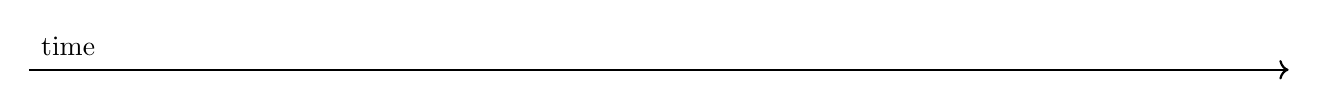
\begin{tikzpicture}
            % Zeit "Time" über dem Pfeil links positionieren
            \node at (-7.5, 0.3) {time}; % Text "Time"
            \draw[->, thick] (-8, 0) -- (8, 0); % Pfeil von ganz links nach ganz rechts
        \end{tikzpicture}
    \end{minipage}

    % Beschriftung unter dem Grid
    \vspace{0.5cm}
    \caption{Limitation of \ac{TEP}-Net \cite{tepNet2024}. The introduced approach is a single-frame-based model. Therefore, no temporal context can be captured, which leads to uncertainty in prediction when driving over a switch.
    All images are from \cite{limitaion_youtube_video}. A YouTube video, which is also used by RailSem19. It is ensured that none of the frames are included in the dataset, creating a fair test scenario.}
    \label{fig:limitationSwitch}
\end{figure}

There are two approaches suggested in \cite{tepNet2024}.
The first one includes integrating a confidence score to tell if the model is in a scenario where it is prone to become unreliable.
The second suggested approach is more complete.
It would encounter the temporal component by implementing a model like a \ac{RNN}, that can capture temporal information.
However, \cite{tepNet2024} states that there is no public temporal dataset available, which fits this task.
To the best of the author knowledge, this statement is correct.
Therefore, a corresponding dataset must also be created, if this approach is pursued.

%%%%%%%%%%%%%%%%%%%%%%%%%%%%%%%%%%%%%%%%%%%%%%%%%%%%%%%%%%%%%%%%%%

%%%%%%%%%%%%%%%%%%%%% temporal network architectures %%%%%%%%%%%%%%%%%%%%%

\clearpage
\section{Temporal Model Architectures}
\label{sec:temporalModelArchitecture}

blidtext

\begin{itemize}
    \item LSTM -> 1 Seite
    \item GRU -> 1 Seite
    \item ...
\end{itemize}

%%%%%%%%%%%%%%%%%%%%%%%%%%%%%%%%%%%%%%%%%%%%%%%%%%%%%%%%%%%%%%%%%%

%%%%%%%%%%%%%%%%%%%%% Datasets %%%%%%%%%%%%%%%%%%%%%

\clearpage                                                       % Beginne neue Seite
\section{Datasets}
\label{sec:datasets}

Datasets are essential for the development of autonomous driving systems, particularly for training and testing algorithms or neural networks.
Typically, raw sensor data is collected from real-world driving scenarios, providing a realistic environment that reflects potential situations the system may encounter in future applications.
This allows for more accurate modeling and evaluation of the system's performance under real conditions.
A common approach to solving problems in autonomous driving systems is using vision-based machine learning algorithms ~\cite[S.~1221]{railsem19dataset}.
These applications typically rely on camera-based data to address various challenges ~\cite[S.~1221]{railsem19dataset}.

Since, autonomous vehicles are increasingly considered a groundbreaking technology of the future \cite{FraunhoferInstituteforCognitiveSystemsIKS} a lot of work is put in the development of such systems.
However often the main focus of this quickly evolving field is on road vehicles, like cars or trucks.
Therefore, most publicly available datasets focus on this application and primarily reflect scenarios in road traffic \cite[S.~1221]{railsem19dataset}.

\subsubsection{Classification Datasets}

There are a couple of public datasets for different \ac{CV} applications. The data of the following datasets are especially gathered for classification tasks.

% ---------------------------------------- Table: Datasets for Classification ----------------------------------------
\begin{table}[H]
\centering
\caption{Datasets for Classification}\label{tab_datsets_classification}
\begin{tabular}{| p{0.3\linewidth} | p{0.3\linewidth} | p{0.3\linewidth} |}\hline
Dataset & Labels & Number of relevant images\\\hline
CIFAR 100 & trains & 600\\\hline
PASCAL VOC2012 & trains & 544\\\hline
Microsoft COCO & trains & 3745\\\hline
1000 ImageNet & \begin{tabular}[c]{@{}l@{}}electric\_locomotive, \\ steam\_locomotive, \\ bullet\_train\end{tabular} & 6722\\\hline
Open Images Dataset V4 & train & 9284\\\hline
\end{tabular}
\end{table}
% --------------------------------------------------------------------------------------------------------------------


\textit{CIFAR 100} dataset \cite{cifar100} consists of small images with pixel size 32x32. This dataset includes 600 images with the label \textit{trains}.
In \textit{PASCAL VOC2012} \cite{pascal2015} there are 544 images labeled \textit{trains}.
\textit{Microsoft COCO} \cite{Lin2014MicrosoftCC} has 3745 images with the class \textit{trains}.
Additionally, there are classes like \textit{traffic lights} and \textit{stop sign}, however theses are not useful to the task of this work because they are from the street domain and not the rail domain.
\textit{1000 ImageNet} \cite{ImageNet2015} includes labels like \textit{electric\_locomotive} (4330 images), \textit{steam\_locomotive} (1187 images) and \textit{bullet\_train} (1205 images).
\textit{Open Images Dataset V4} \cite{openImagesV42018} consists of more than 9.2 million images, annotated with bounding boxes.
Included are 10506 \textit{train}-labels in 9284 images.
However, there are no other significant labels relevant to the rail domain.
Additionally, the dataset contains labels for toy trains, which could pose potential challenges.

\subsubsection{Semantic Segmentation}

Semantic segmentation labels are often refereed to as dense or pixel-wise annotated data.
These datasets are characterized by the fact that each pixel in their images is assigned to a class.

% ---------------------------------------- Table: Datasets for Semantic Segmentation ----------------------------------------
\begin{table}[H]
\centering
\caption{Datasets for Semantic Segmentation}\label{tab_datasets_semanticSegmentation}
\begin{tabular}{| p{0.3\linewidth} | p{0.3\linewidth} | p{0.3\linewidth} |}\hline
Dataset & Labels & Number of relevant images\\\hline
Cityscapes & rail track, train & 284\\\hline
Mapillary Vistas & \begin{tabular}[c]{@{}l@{}}construction-flat-rail-track, \\ object-vehicle-on-rails\end{tabular} & 710\\\hline
COCO-Stuff & platform, railroads, train & 8615\\\hline
KITTI & rail tracks, train & 65\\\hline
\end{tabular}
\end{table}
% ---------------------------------------------------------------------------------------------------------------------------

The \textit{Cityscapes} dataset \cite{cityscapes2016} is commonly used for benchmarks when it comes to road scenes.
It has 35 different labels of which two are \textit{rail track} (131 labels in 117 images) and \textit{train} (194 labels in 167 images).
The \textit{rail track} does not differ between the rails and track bed.
\textit{Mapillary Vistas} \cite{mapillaryVistas2017} also has more labels, but again only two are rail related ones.
\textit{construction-flat-rail-track} is annotated in 710 images and \textit{object-vehicle-on-rails} occurs 272 times.
\textit{COCO-Stuff dataset} \cite{COCO-StuffDataset} includes the same 182 classes like the \textit{Microsoft COCO} \cite{Lin2014MicrosoftCC} but as dense labels.
The rail relevant ones are \textit{railroad} (2839) and \textit{train} (4761).
There is a third rail related label \textit{platform}, however this is a very general label because this can by any plane.
\textit{KITTI} \cite{kittiDataset2018} has the same dense labels like \textit{Cityscapes} \cite{cityscapes2016}.
Likewise, the rail relevant ones are 47 \textit{rail track} and 18 \textit{train} labels.

% Problems with general datsets
These are commonly used datasets in \ac{CV} tasks. However there are there are three main issues when it comes to solving the track prediction use case presented in this work.
Firstly, there is not enough data because the amount of included rail relevant labels is relatively low in each dataset.
Secondly, the labels present are not suitable for training a track prediction algorithm. In this case only the rails, rail tracks or track beds are needed.
Thirdly, the images of the presented datasets are taken out of passengers and pedestrian views. Additionally there are some road views \cite{Hadded.2022}.

% Birds eye views und sign datasets
The datasets mentioned before are very general with a vast amount of different labels.
However there are some datasets specially captured for the rail domain.
As with the other datasets, it is important to consider what specific tasks the datasets are intended to be used for.
There are some datasets captured in the birds eye view to detect damages like cracks in rails \cite{rail5k2021} \cite{ma2024cross} or even some to detect garbage in grooved rails \cite{Huang_2021}. Then there are datasets in ego-perspective of the train driver like \textit{FRSign} \cite{Harb2020FRSignAL} or \textit{GERALD} \cite{leibner2023gerald}, which are created for detecting different traffic lights on French and German railways.

% Überleitung mit Perspective Problem zu ego-perspective datasets
This work deals with Rail Track Prediction, so the system should predict the direction of the track in front of the train. For this particular use case it is most advantages when the dataset is recorded out of the driver cabin in ego-perspective, because it offers a clear sight of the rails in front of the train. Therefore the data has to reflect scenarios, which are comparable. Since the view of the captured images represents a key factor, the before mentioned dataset become unsuitable. An additional reason why these datasets cannot be used for this work is the fact that they are created for different use cases.
Other datasets which deal with the perception in a rail domain environment and are captured in the right perspective are discussed in the following paragraphs.

% ================= Richtige datasets =================

% RailSem19
\subsubsection{RailSem19}
\textit{RailSem19} \cite{railsem19dataset} is the first publicly available dataset fitted for environments in the rail domain. It consists of 8500 annotated images which are gathered from YouTube videos. All of these images are captured in the ego perspective of the train driver, which makes it suitable for the use case of this work. Additionally there are both bounding box labels and dense labels included for object detection and semantic segmentation. The bounding box labels are: \textit{guard-rail; rail; traffic-signal-front; traffic-signal-back; traffic-sign-front; crossing; train; platform; buffer-stop; switch-indicator; switch-static; switch-left; switch-right; switch-unknown}. Important for predicting the direction of the train are the switch labels, because  it gives valuable information. The \textit{switch-unknown} label is used when there is a switch visible but it is unclear in which direction the train would proceed. The presents of this label is mainly due to the high noise levels of the images of YouTube videos.
The dense labels of RailSem19 are: \textit{road; sidewalk; construction; tram-track; fence; pole; traffic-light; traffic-sign; vegetation; terrain; sky; human; rail-track; car; truck; track-bed; on-rails; rail-raised; rail-embedded; void}. In the case of dense labels the labels \textit{tram-track; rail-track; track-bed; on-rails; rail-raised; rail-embedded} are of importance for predicting the direction of trains and trams.
Another advantage is that very diverse environments have been used for this dataset. The creators of \textit{RailSem19} took images from 38 different countries in all four seasons and weather conditions. Additionally, the focus was not only on rails but also on trams, providing a very diverse reflection of rail scenarios and not limiting the use on a specific use case.

\begin{figure}[H]
    \centering
    
    % Erste Reihe
    \begin{subfigure}{0.328\textwidth}
        \includegraphics[width=\linewidth]{PICs/datasets/RailSem19_dataset/RailSem19_Bild1.png}
    \end{subfigure}
    \hfill
    \begin{subfigure}{0.328\textwidth}
        \includegraphics[width=\linewidth]{PICs/datasets/RailSem19_dataset/RailSem19_Bild2.png}
    \end{subfigure}
    \hfill
    \begin{subfigure}{0.328\textwidth}
        \includegraphics[width=\linewidth]{PICs/datasets/RailSem19_dataset/RailSem19_Bild3.png}
    \end{subfigure}

    \vspace{0.1cm} % Größerer Abstand zwischen den Reihen

    % Zweite Reihe
    \begin{subfigure}{0.328\textwidth}
        \includegraphics[width=\linewidth]{PICs/datasets/RailSem19_dataset/RailSem19_Bild1_GT.png}
    \end{subfigure}
    \hfill
    \begin{subfigure}{0.328\textwidth}
        \includegraphics[width=\linewidth]{PICs/datasets/RailSem19_dataset/RailSem19_Bild2_GT.png}
    \end{subfigure}
    \hfill
    \begin{subfigure}{0.328\textwidth}
        \includegraphics[width=\linewidth]{PICs/datasets/RailSem19_dataset/RailSem19_Bild3_GT.png}
    \end{subfigure}

    \caption{RailSem19 dataset examples. First row raw images. Second row dense \ac{GT} \cite{railsem19dataset}.}
    \label{fig:railSem19-images-denseLabels}
\end{figure}

%RailVID
\subsubsection{RailVID}
\label{subsubsec:railVID}
Another dataset that focuses on the detection of rails is the \textit{RailVID} dataset \cite{yuan2022railvid}. The goal of this project is to detect rail tracks and obstacles on the rails, which can lead to possible hazardous situations. With a functioning system, fully automatic train operation is aimed for. The \textit{RailVID} dataset is a collection of 1071 images with the following labels: \textit{background, railway, car, people}. Since, the area of application is on the "Suzhou Rail Transit Line 1" in Jiangsu Province, China all data is captured there. \textit{RailVID} is a collection of infrared data captured with the AT615X infrared thermal instrument from InfiRay. The decision to use infrared data and not RGB images is because it is more robust against challenging imaging conditions, like darkness at night, fog, rain and direct light disturbance.
Since, this dataset only consists of infrared data and in this work \ac{RGB} data should be used, \textit{RailVID} cannot be used fro training. An additional issue is, that the dataset is recorded only on a specific Chinese line. This is advantageous for this particular use case, but it could become an issue if the system were to be deployed elsewhere.

\begin{figure}[H]
    \centering
    \begin{subfigure}{0.24\textwidth}
        \centering
        \includegraphics[width=\linewidth]{PICs/datasets/railVID_dataset/railVID_data.png}
    \end{subfigure}
    \hfill
    \begin{subfigure}{0.24\textwidth}
        \centering
        \includegraphics[width=\linewidth]{PICs/datasets/railVID_dataset/railVID_label.png}
    \end{subfigure}
    \hfill
    \begin{subfigure}{0.24\textwidth}
        \centering
        \includegraphics[width=\linewidth]{PICs/datasets/railVID_dataset/railVID_switch.png}
    \end{subfigure}
    \hfill
    \begin{subfigure}{0.24\textwidth}
        \centering
        \includegraphics[width=\linewidth]{PICs/datasets/railVID_dataset/railVID_switch_label.png}
    \end{subfigure}
    \caption{Example images and \ac{GT} of RailVID dataset \cite{yuan2022railvid}}
    \label{fig:railVID_dataset_images}
\end{figure}

% RailSet
\subsubsection{RailSet}
\cite{railSet2022} and \cite{hadded2022application} presented the \textit{RailSet} dataset,
which is divided into two sub sets: RailSet-Seg for segmentation and RailSet-Ano for anomaly detection \cite{railSet2022}.
Both of them are captured in the ego perspective of the train driver \cite{railSet2022} \cite{hadded2022application}.
The idea is to firstly detect the railways using semantic segmentation and secondly using positional information of the prediction for the creation of the anomaly dataset \cite{railSet2022}.
RailSet-Ano is a collection of 1100 images of railway defects like rail discontinuity and holes in the rail bed.
Some anomalies are taken from a other images and pasted on images of RailSet-Seg and RailSem19 dataset others are generated with a network \cite{railSet2022}.
Since, RailSet-Ano deals with a different use case than the one in this work, this particular data cannot be used.

On the other hand, RailSet-Seg fits the problem. It consists of 6600 images of normal situations.
The images are collected from 23 YouTube videos with a collective duration of 15 hours. It includes two labels: \textit{rail} and \textit{rail-track}.
Besides the use of  RailSet-Seg for the creation of RailSet-Ano, an additional motivation is to include more complex scenes of the rail domain than RailSem19.
That is why the focus of RailSet lies on scenarios with poor weather conditions or lighting conditions.
Furthermore, images are included in which the rails are not visible at all, like in tunnels without lighting or in snowy scenes.
Additionally, it was ensured that the videos were recorded by different cameras and from different mounting positions \cite{railSet2022} \cite{hadded2022application}. 

An advantage of this dataset is that it can be joined with RailSem19, when combining four specific labels.
\textit{trackbed} and \textit{rail-track} from RailSem19 have to be transformed into RailSet's \textit{rail-track} label and \textit{rail-raised} and \textit{rail-embedded} become the \textit{rail} label.
This method leads to more data for the training and validation which could be an advantage.
However, it also shows the disadvantage of this dataset for the specific use case of this work. 
RailSet exclusively addresses railway and not tram scenes \cite{hadded2022application}.
Since, the goal is to target a broad applicability, leaning towards tram scenes this dataset is not used for this work.

% Bild von RailSet
\begin{figure}[H]
    \centering
    \begin{subfigure}{0.3\textwidth}
        \centering
        \includegraphics[width=\linewidth,height=5cm,keepaspectratio]{PICs/datasets/RailSet_dataset/RailSet_image.png}
        \caption{}
        \label{fig:RailSet-Seg_example_image_GT_a}
    \end{subfigure}
    \hspace*{0.02\textwidth} % Abstand manuell steuern
    \begin{subfigure}{0.3\textwidth}
        \centering
        \includegraphics[width=\linewidth,height=5cm,keepaspectratio]{PICs/datasets/RailSet_dataset/RailSet_GT_rails.png}
        \caption{}
        \label{fig:RailSet-Seg_example_image_GT_b}
    \end{subfigure}
    \hspace*{0.02\textwidth} % Abstand manuell steuern
    \begin{subfigure}{0.3\textwidth}
        \centering
        \includegraphics[width=\linewidth,height=5cm,keepaspectratio]{PICs/datasets/RailSet_dataset/RailSet_GT_rails&rail-track.png}
        \caption{}
        \label{fig:RailSet-Seg_example_image_GT_c}
    \end{subfigure}
    \caption{RailSet-Seg example with annotations \cite{railSet2022} \cite{hadded2022application}: \textbf{(a)} raw-image, \textbf{(b)} rail class, \textbf{(c)} rail and rail-track class}
    \label{fig:RailSet-Seg_example_image_GT}
\end{figure}


% RSDS
\subsubsection{RSDS}
The creators of the \ac{RSDS} \cite{railNet2019}, tried to solve the railroad detection problem with a segmentation approach. Because there was no publicly available dataset for this task at the time, they had to construct their own. \ac{RSDS} is captured from the ego perspective of the train driver and is a collection of 3000 images. They used 2500 for training, 200 for validation and 300 for testing. The dataset only includes one \textit{railroad} label. It is described that the labels only incorporate pixels between the two rails and intentionally ignore railway sleepers outside this area. Images are of size 1920 x 1080.
Although it is not mentioned in the paper, it seems as if all images of \ac{RSDS} are captured from a specific rail line in China. Additionally, from the images in the paper alone one can tell that this particular rail line has very distinctive structural characteristics. The colors are bright and it seems like the area between the rails is mostly concrete, which is unusual for most railways. \ref{fig:RSDS_example_image_GT} shows that structures besides the rails are specific too.
One additional detail of this dataset, which can present a disadvantage for this work, is that switches are not addressed.
Since this dataset only covers very specific railroads with unique characteristics and additionally does not address switches or other situations where the track splits, \ac{RSDS} is not further considered for this work.

% Bild von RSDS
\begin{figure}[H]
    \centering
    \begin{subfigure}{0.45\textwidth}
        \includegraphics[width=\linewidth,height=5cm,keepaspectratio]{PICs/datasets/RSDS_dataset/RSDS_image.png}
        \caption{}
        \label{fig:RSDS_example_image_GT_a}
    \end{subfigure}
    \hfill
    \begin{subfigure}{0.45\textwidth}
        \includegraphics[width=\linewidth,height=5cm,keepaspectratio]{PICs/datasets/RSDS_dataset/RSDS_GT.png}
        \caption{}
        \label{fig:RSDS_example_image_GT_b}
    \end{subfigure}
    \caption{\ac{RSDS} example with annotation \cite{railNet2019}: \textbf{(a)} raw-image, \textbf{(b)} ground truth}
    \label{fig:RSDS_example_image_GT}
\end{figure}

% Rail-DB
\subsubsection{Rail-DB}
A very similar dataset is Rail-DB \cite{li2022rail}.
This dataset is a collection of 7432 images, which are taken from 15 videos.
The labels in this dataset are consist of poly lines, which represent all existing rails in an image.
Additionally the the poly lines all have different classes. This way there is not only one rail class, but as many classes as there are rails in one image.
The labeling policy specifies that the central rails are marked with the annotations 1 and 2.
Additional rails are labeled with rising numbers.
Since this dataset includes poly lines and not binary masks, this dataset can be used for training line detection algorithms.
Compared to \ac{RSDS}, this dataset includes not only lines and curves, but also rail switches.
Additionally, the images are taken in various conditions and scenes.
\ref{fig:Rail-DB-dataset_images_annotated} shows example images of Rail-DB's different scenes.
However, it seems that the images again have very specific characteristics like in \ac{RSDS}.
\ref{fig:Rail-DB-dataset_images_annotated} also shows, that all images are captured on a Chinese line.
Even though \cite{li2022rail} presents a very interesting approach for solving the rail detection problem,
because of the before mentioned specific characteristics it is not used for this work. Even the author of \cite{li2022rail} states in the GitHub repository \cite{railNet2022GitHub},
that this project fails to generalize on example videos, where the scene looks different from the one the dataset is captured on.

\begin{figure}[H]
    \centering
    \begin{subfigure}{0.328\textwidth}
        \centering
        \includegraphics[width=\linewidth,height=5cm,keepaspectratio]{PICs/datasets/railDB_dataset/railDB_fog.png}
    \end{subfigure}
    %\hspace*{0.02\textwidth} % Abstand manuell steuern
    \hfill
    \begin{subfigure}{0.328\textwidth}
        \centering
        \includegraphics[width=\linewidth,height=5cm,keepaspectratio]{PICs/datasets/railDB_dataset/railDB_switch.png}
    \end{subfigure}
    %\hspace*{0.02\textwidth} % Abstand manuell steuern
    \hfill
    \begin{subfigure}{0.328\textwidth}
        \centering
        \includegraphics[width=\linewidth,height=5cm,keepaspectratio]{PICs/datasets/railDB_dataset/railDB_night.png}
    \end{subfigure}
    \caption{Rail-DB \cite{li2022rail} images with annotations in different conditions}
    \label{fig:Rail-DB-dataset_images_annotated}
\end{figure}


% OSDaR23
\subsubsection{OSDaR23}
Another dataset it the OSDaR23 \cite{oSDaR23}.
This dataset is a collection of 21 sequences, which are split into 45 subsequences.
Several sequences are short ones with 10 frames each, some are longer with 40 to 100 frames.
In total there are 1534 labeled scenes in this dataset.
Since, OSDaR23 is captured with 9 cameras (\ac{RGB} and \ac{IR}) in different angles, one lidar and one radar sensor, the total number of frames are 1534 * 11 = 16874.
Additionally, position and acceleration sensors are used.
Because also lidar and radar is used, this dataset offers 3D data as well.
OSDaR23 consists of 20 different labels.
These labels include the rail context, like \textit{track}, \textit{switch} or \textit{train} and the environment, like \textit{person}, \textit{animal}, \textit{bicycle}, \textit{smoke}, \textit{flame} or \textit{crowd}.
The annotations for the environment can be used for safety applications.
For more details please refer to \textit{TABLE V} in \cite{oSDaR23}.
\ref{fig:OSDaR23_captured_data} shows the 11 different frames of each sensor and \ref{fig:OSDaR23_annotated} shows an example of an annotated scene.
As illustrated in \ref{fig:OSDaR23_annotated} the \textit{track} label and the \textit{switch} label only offers positional information about their presents, but do not include any information on the direction of the train.
Furthermore, there is no information that distinguishes the train rails from the adjacent rails.
Therefore OSDaR23 can only be used for the detection of rails, but not the track prediction.
Moreover, the capturing of this dataset only took place on rail roads in Hamburg, Germany.
No tram scenes are included.
Due to the necessity of re-labeling for this work and the fact that only data from Hamburg is offered, OSDaR23 is not used.


% captured data
\begin{figure}[H]
    \centering
    % Erstes Bild
    \begin{subfigure}{\textwidth}
        \centering
        \includegraphics[width=0.5\textwidth]{PICs/datasets/OSDaR23_dataset/camerasetup_high_res_cameras.png}
    \end{subfigure}

    % Zweites Bild
    \begin{subfigure}{\textwidth}
        \centering
        \includegraphics[width=0.5\textwidth]{PICs/datasets/OSDaR23_dataset/camerasetup_low_res_cameras.png}
    \end{subfigure}

    % Drittes Bild
    \begin{subfigure}{\textwidth}
        \centering
        \includegraphics[width=0.5\textwidth]{PICs/datasets/OSDaR23_dataset/camerasetup_IR.png}
    \end{subfigure}

    % Viertes Bild
    \begin{subfigure}{\textwidth}
        \centering
        \includegraphics[width=0.5\textwidth]{PICs/datasets/OSDaR23_dataset/camerasetup_Lidar_Radar.png}
    \end{subfigure}
    
    \caption{OSDaR23 data from all different sensors \cite{oSDaR23}}
    \label{fig:OSDaR23_captured_data}
\end{figure}

% labeled scene
\begin{figure}[H]
    \centering
    % Erste Reihe: Zwei Bilder nebeneinander
    \begin{subfigure}{0.45\textwidth}
        \centering
        \includegraphics[width=\textwidth]{PICs/datasets/OSDaR23_dataset/labeled_image.png}
        \caption{\ac{RGB} center camera}
    \end{subfigure}%
    \hspace{0.05\textwidth}
    \begin{subfigure}{0.45\textwidth}
        \centering
        \includegraphics[width=\textwidth]{PICs/datasets/OSDaR23_dataset/labeled_3D.png}
        \caption{merged lidar point cloud}
    \end{subfigure}

    \vspace{0.5cm} % Abstand zwischen den Reihen

    % Zweite Reihe: Zwei Bilder nebeneinander
    \begin{subfigure}{0.45\textwidth}
        \centering
        \includegraphics[width=\textwidth]{PICs/datasets/OSDaR23_dataset/labeled_IR.png}
        \caption{IR center camera}
    \end{subfigure}%
    \hspace{0.05\textwidth}
    \begin{subfigure}{0.45\textwidth}
        \centering
        \includegraphics[width=\textwidth]{PICs/datasets/OSDaR23_dataset/labeled_Radar.png}
        \caption{Radar (zoomed)}
    \end{subfigure}
    
    \caption{OSDaR23 annotated scene \cite{oSDaR23}}
    \label{fig:OSDaR23_annotated}
\end{figure}



\begin{figure}[H]
    \centering
    % Erste Reihe: Zwei Bilder nebeneinander, feste Breite und Höhe
    \begin{subfigure}{0.45\textwidth}
        \centering
        \includegraphics[width=0.9\textwidth,height=5cm]{PICs/datasets/OSDaR23_dataset/labeled_image.png}
        \caption{Bild 1}
    \end{subfigure}%
    \hspace{0.05\textwidth}
    \begin{subfigure}{0.45\textwidth}
        \centering
        \includegraphics[width=0.9\textwidth,height=5cm]{PICs/datasets/OSDaR23_dataset/labeled_3D.png}
        \caption{Bild 2}
    \end{subfigure}

    \vspace{0.5cm} % Abstand zwischen den Reihen

    % Zweite Reihe: Zwei Bilder nebeneinander, gleiche feste Breite und Höhe
    \begin{subfigure}{0.45\textwidth}
        \centering
        \includegraphics[width=0.9\textwidth,height=5cm]{PICs/datasets/OSDaR23_dataset/labeled_IR.png}
        \caption{Bild 3}
    \end{subfigure}%
    \hspace{0.05\textwidth}
    \begin{subfigure}{0.45\textwidth}
        \centering
        \includegraphics[width=0.9\textwidth,height=5cm]{PICs/datasets/OSDaR23_dataset/labeled_Radar.png}
        \caption{Bild 4}
    \end{subfigure}
    
    \caption{OSDaR23 labels skaliert}
\end{figure}

% TEP-Net annotations
\subsubsection{TEP-Net dataset}
\label{subsubsec:TEP-Net_dataset}

\cite{tepNet2024} presents the \ac{TEP}-Net dataset.
The problem this paper aims to solve is rail track prediction.
This differs from all previously mentioned datasets.
No dataset but \cite{tepNet2024} provides information, which distinguishes possible rails in the image from the one the train actually follows.
Since RailSem19 is the most popular dataset in the rail domain, it is used as initial point.
A total of 7917 images were taken from RailSem19.
The remaining 583 were excluded because they are taken from unusual perspectives or it is unclear which track the train is on or would continue on.
Examples of such images are shown in \ref{tep-net_aussortiert}.
These images are excluded simply by not annotating them.
For annotation a new labeling format is created.
Two classes \textit{rail\_right} and \textit{rail\_left} give information about where the tracks of the train  run.
All other rails which might be in the image are ignored.
These two classes consist of poly lines, which are annotated by the corresponding x and y pixel coordinates of the image.
Only the tracks on which the train is located are labeled.
Even if a switch appears in the image and the train would travel over it, only the tracks in the correct direction are further labeled.
This way, switches are indirectly included in this dataset, providing information on the direction a train would continue, even though there is no explicit label for switches.
The poly lines start from lowest pixel row of the images and extend up to a specific horizon line.
Above this horizon further labeling is not possible.
This may occur for various reasons.
The first reason can be an obstruction of the view by the environment or other trains, as shown in \ref{fig:tep-net-annotated-images}.
Since the images are sourced from YouTube videos, it is also possible that the resolution becomes too low in the distance for separately identifying both rails.
Another reason is when it is not possible to determine the direction in which the track continues based on a switch present in an image.
This can happen due to low resolution or unfortunate camera angles.
These cases may be labeled as \textit{switch-unknown} in the original RailSem19 dataset for example.
Here, the polylines stop before the switch.
The polylines from this annotation can then be converted into several different labels using preprocessing algorithms.
On one hand, they can be directly used as polylines.
On the other hand, they can be transformed into a mask for segmentation tasks by filling in the area between the lines.
A third application would be to convert this mask into a grid for classification tasks.

\begin{figure}[H]
    \centering
    \includegraphics[width=\linewidth]{PICs/datasets/TEP_dataset/TEP-Net dataset bilder aussortiert.png}
    \caption{Examples images from RailSem19, which are not included in the \ac{TEP}-Net dataset due to unclear circumstances about the trains direction. \cite{tepNet2024}}
    \label{tep-net_aussortiert}
\end{figure}


\begin{figure}[H]
    \centering
    
    % Erste Reihe
    \begin{subfigure}{0.328\textwidth}
        \includegraphics[width=\linewidth]{PICs/datasets/TEP_dataset/annotated_rs00007.jpg}
    \end{subfigure}
    \hfill
    \begin{subfigure}{0.328\textwidth}
        \includegraphics[width=\linewidth]{PICs/datasets/TEP_dataset/annotated_rs00107.jpg}
    \end{subfigure}
    \hfill
    \begin{subfigure}{0.328\textwidth}
        \includegraphics[width=\linewidth]{PICs/datasets/TEP_dataset/annotated_rs00244.jpg}
    \end{subfigure}

    \vspace{0.1cm} % Größerer Abstand zwischen den Reihen

    % Zweite Reihe
    \begin{subfigure}{0.328\textwidth}
        \includegraphics[width=\linewidth]{PICs/datasets/TEP_dataset/annotated_rs00284.jpg}
    \end{subfigure}
    \hfill
    \begin{subfigure}{0.328\textwidth}
        \includegraphics[width=\linewidth]{PICs/datasets/TEP_dataset/annotated_rs00256.jpg}
    \end{subfigure}
    \hfill
    \begin{subfigure}{0.328\textwidth}
        \includegraphics[width=\linewidth]{PICs/datasets/TEP_dataset/annotated_rs00198.jpg}
    \end{subfigure}

    \caption{\ac{TEP}-Net dataset example images with annotation \cite{tepNet2024}}
    \label{fig:tep-net-annotated-images}
\end{figure}

\textbf{notes wo alles ist}

\begin{itemize}
    \item Railroad Segmentation Dataset (RSDS) --> in RailNet: A Segmentation Network for Railroad Detection fertig
    \item RailSem19 in RailSem19 fertig
    \item RailVID in RailVID fertig
    \item RailSet in RailSet \& Application of Rail Segmentation in the Monitoring of Autonomous Train’s Frontal Environment fertig
    \item Rail-DB (compared to RSDS) --> Rail Detection: An Efficient Row-based Network and A New Benchmark fertig
    \item OSDaR23 in OSDaR23: Open Sensor Data for Rail 2023 fertig
    \item TEP-net dataset fertig
    \item
    \item RailSet -> Segmentation \& Anomaly detection
    \item Application of Rail Segmentation in the Monitoring of Autonomous Train’s Frontal Environment -> RailSegmentation (only rails and trackbed)
\end{itemize}

%%%%%%%%%%%%%%%%%%%%%%%%%%%%%%%%%%%%%%%%%%%%%%%%%%%%%%%%%%%%%%%%%%


%%%%%%%%%%%%%%%%%%%%%%%%%%%%%%%%%%%%%%%%%%%%%%%%%%%%%%%%%%%%%%%%%%
%%%%%%%%%%%%%%%%%%%%%%%%%%% Methodology %%%%%%%%%%%%%%%%%%%%%%%%%%
\clearpage                                                       % Beginne neue Seite

% Include the first subsection from an external file
\chapter{Methodology}
\label{sec:methodology}
blindtext

\section{Datasets}
blindtext

\subsection{RailSem19 and used subsets}
blindtext

\subsection{vielleicht: Rail-DB for multi rail setection}
blindtext

\subsection{used annotations}
blindtext

\section{Switch evaluation dataset}
blindtext

\section{labeling task for temporal models}

\subsubsection{CVAT}
\subsubsection{Autolabler}
blindtext

%%%%%%%%%%%%%%%%%%%%% Data augmentation %%%%%%%%%%%%%%%%%%%%%

\section{Data augmentation}
\label{sec:dataaugmentation}

This section describes both the data augmentation strategy for training and the cropping augmentation for inference.

\subsubsection{Data augmentation for Training}

Three data augmentation techniques are implemented to train the model.
The first two are commonly used in CV tasks, including random horizontal flips and traditional image adjustments like brightness, contrast, saturation, and hue variations.
For this, the standard ColorJitter method from PyTorch is used \cite{pytorch_colorJitter_docu}.
The third augmentation is the cropping mechanism, which reduces the image to the most relevant part.
Randomness is also introduced to enhance generalization.

\autoref{fig:tepNet_dataaugmentation} visualizes the cropping algorithm steps schematically.
At first, there are two green lines, which follow the train's ego-path and represent the \ac{GT} in the form of polylines.
Then the yellow rectangle is computed with this information, being the smallest possible rectangle around the \ac{GT}.
In the next step, the orange box, the start pixels of the rails \ac{GT} are centered by expanding the yellow borders in one direction.
Important to mention is that in this tailored dataset the rails always begin in the first row at the bottom of each image.
After that margins are added shown by the red rectangle.
These margins are predefined with hyperparameters.
After calculating the borders of the outermost box variability is added to enhance generalization and prevent biases.
The left, right, and top borders are moved by a distance calculated with a normal distribution, which is defined by hyperparameters.
This introduced variability follows the policy, which ensures that the starting pixels of the rails at the bottom stay in the cropped image.
\autoref{fig:tepNet_dataaugmentation} illustrates four augmented variations of the top image in the bottom row.

\begin{figure}[H]
    \centering
    \includegraphics[width=0.6\linewidth]{PICs/Baselinepaper/data_augmenation.jpg}
    \caption{Data augmentation of \ac{TEP}-Net \cite{tepNet2024}, including the image horizontal flips, the color variations and the cropping mechanism.}
    \label{fig:tepNet_dataaugmentation}
\end{figure}

\subsubsection{Cropping in inference}

In \cite{tepNet2024} only cropped images are used for training the model to minimize the images to their most relevant \ac{ROI}.
For training and validating the model on the dataset, the \ac{GT} allows the computation of crop coordinates (left, top, right).
However, \ac{GT} data is unavailable in practical applications like video inference.
As a result, the crop coordinates must be, either predefined by a user or computed on the fly.

In a real-world application the ROI in the images changes, even when the camera is mounted in a fixed position.
Because of these perspective shifts when the train drives right or left turns, it easily can become unsustainable to have predetermined crop coordinates.
\autoref{fig:perspective_shifts} visualizes these perspective shifts.
The tighter the curve, the worse the shift.
The approach of \cite{tepNet2024} to solve this particular problem is the so-called "Autocrop".
This developed technique starts with the whole image, so the initial crop cords are the image borders.
After the initialization, the three coordinates (left, top, right) are updated according to the prediction of every new frame.
In more detail, new coordinates are calculated with a running average of the smallest rectangle around the prediction plus the predefined margins from the training.

\begin{figure}[H]
    \centering
    \includegraphics[width=0.6\linewidth]{PICs/Baselinepaper/perspective_shifts.jpg}
    \caption{Example of perspective shifts with three different scenarios: left curve, right curve and straight rail \cite{tepNet2024}.}
    \label{fig:perspective_shifts}
\end{figure}

%%%%%%%%%%%%%%%%%%%%%%%%%%%%%%%%%%%%%%%%%%%%%%%%%%%%%%%%%%%%%%%%%%

%%%%%%%%%%%%%%%%%%%%% Baseline model %%%%%%%%%%%%%%%%%%%%%

\input{methodology/baseline_model.tex}

%%%%%%%%%%%%%%%%%%%%%%%%%%%%%%%%%%%%%%%%%%%%%%%%%%%%%%%%%%%%%%%%%%

%%%%%%%%%%%%%%%%%%%%% Loss function %%%%%%%%%%%%%%%%%%%%%

\section{Loss function}
\label{sec:lossFunction}

One of the main contributions of \cite{tepNet2024} is the loss function, which is tailored to the particular problem formulation of the regression-based approach.
Since, this loss function demonstrates to be functional, it is adopted unchanged in this work.
This loss function \autoref{func:combinedLoss} \cite{tepNet2024} consists of two sub-functions, where the outputs are added together, with the $y$-limit loss weighted by a multiplication factor of $\lambda=0.5$ before summing.

\begin{align}
    L = L_{traj} + \lambda \times L_{ylim}
    \label{func:combinedLoss}
\end{align}

The two sub-functions are the trajectory loss $L_{traj}$ and $y$-limit loss $L_{ylim}$.
For the following functions, $\hat{\mathbf{X}}$ and $\mathbf{X}$ represent the predicted and \ac{GT} $x$-values.
These include the points for the left and right rails.
For the $y$-limit, the predicted and \ac{GT} values are $\hat{y}_{lim}$ and $y_{lim}$.

\vspace{1cm}

\noindent \textbf{Trajectory Loss} $L_{traj}$ determines the error between the predicted and actual $x$-values.
To calculate this error, the sum of smoothL1 is used as shown in the numerator \autoref{func:trajectoryLoss}.
This is done with a $\beta_{1} = 0.005$. As shown in figure \autoref{fig:smoothL1}, this function allows a linearly proportional relationship between loss and error.
Additionally, for noise in the data, it includes a smooth transition at zero.

One issue of the front view perspective is the so-called linear perspective effect.
This effect occurs when rails continue into the distance.
The same pixel error represents a small distance when near the camera's capturing point and a larger distance when far away.
This ratio grows linearly the greater the distance to the camera.
To counteract this effect, the results of the $L_{rails}(\hat{\mathbf{X}}_{i},\mathbf{X}_{i})$ are multiplied by the $w_{i}$ factor, which is inversely proportional to the width of the rail.
To prevent distortion of the results due to unreasonable weighting $W_{max}$ is used.
This value is the %95^{\text{th}}
percentile of all $w_{i}$ values from the training set.
This value is around 20 when data augmentation is used.

The $m_{i}$ factor is used to zero out and ignore all values above the $y$-limit.
Furthermore, it is ensured that the averaging of the loss is conducted exclusively over the relevant segment of the track.
This is done by summing all $m_{i}$ values in the denominator of \autoref{func:trajectoryLoss}.

%trajectory loss function
\begin{align}
    L_{traj} = \frac{\sum_{i=1}^H m_{i} \times w_{i} \times L_{rails}(\hat{\mathbf{X}}_{i},\mathbf{X}_{i})}
    {\sum_{i=1}^H m_{i}}
    \label{func:trajectoryLoss}
\end{align}

% smooth L1 error function
\begin{align}
    L_{rails} = \sum_{\substack{r \in \{left, right\}}} SmoothL1(\hat{\mathbf{X}}_{i,r} - \mathbf{X}_{i,r}, \beta_1)
    \label{func:smoothL1_error}
\end{align}

% Smooth L1
\begin{align}
    SmoothL1(x, \beta) = 
    \begin{cases}
        0.5 x^2 / \beta, & \text{if } |x| < \beta \\
        |x| - 0.5 * \beta, & \text{otherwise}
    \end{cases}
    \label{func:smoothL1}
\end{align}

% perspective weight function
\begin{align}
    w_{i} = \min \left( \frac{1}{\mathbf{X}_{i,right} - \mathbf{X}_{i,left}} , W_{max} \right)
    \label{func:perspective_weight}
\end{align}

% making factor
\begin{align}
    m_i = 
    \begin{cases} 
        1 & \text{if } i \leq y_{lim} \times H \\
        0 & \text{otherwise}
    \end{cases}
    \label{func:maskingFactor}
\end{align}

\vspace{1cm}

\noindent \textbf{Y-Limit Loss} $L_{ylim}$ is responsible for calculating the error of the horizon line.
For this sub-function also the $SmoothL1$ loss is taken with a $beta_{2} = 0.015$.
The value of $\beta_{2}$ is chosen to be higher, because of greater inaccuracy of annotations.
Due to images of the dataset stemming from low-resolution YouTube videos, it becomes difficult to accurately label the horizon line, especially when the end of the rail track is located at a significant distance.

\begin{align}
    L_{ylim} = SmoothL1(\hat{y_{lim}} - y_{lim}, \beta_{2})
    \label{func:ylimLoss}
\end{align}

\autoref{fig:smoothL1} shows a plot of the \autoref{func:smoothL1} being the $SmoothL1$ Loss function which is widely used in the literature.

\vspace{1cm}

\begin{figure}[H]
    \centering
    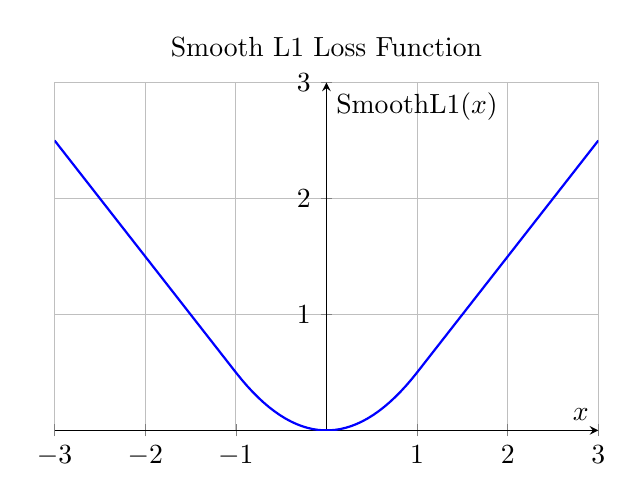
\begin{tikzpicture}
        \begin{axis}[
            title={Smooth L1 Loss Function},
            xlabel={$x$},
            ylabel={SmoothL1($x$)},
            grid=major,
            domain=-3:3, % Bereich der x-Achse
            samples=100, % Anzahl der Punkte
            axis lines=middle, % Achsen durch die Mitte
            %xmin=-3, xmax=3, % Zoom Bereich auf der x-Achse
            width=0.7\textwidth, % Breitere Grafik
            height=6cm, % Schmalere Höhe der Grafik
            ymin=0.0, ymax=3, % Zoom Bereich auf der y-Achse
        ]
            % SmoothL1-Funktion
            \addplot[
                blue, 
                thick
            %]{abs(x) < 0.005 ? 0.5 * (x^2) / 0.005 : abs(x) - 0.5 * 0.005};
            ]{(abs(x) < 1) * (0.5 * x^2) + (abs(x) >= 1) * (abs(x) - 0.5)};
        \end{axis}
    \end{tikzpicture}
    \caption{$SmoothL1$ Loss Funktion}
    \label{fig:smoothL1}
\end{figure}


%%%%%%%%%%%%%%%%%%%%%%%%%%%%%%%%%%%%%%%%%%%%%%%%%%%%%%%%%%%%%%%%%%

%%%%%%%%%%%%%%%%%%%%% Setup used for Training CNNs %%%%%%%%%%%%%%%%%%%%%

\section{Setup used for Training CNNs}
\label{sec:trainigsSetup}

% Hardware (GPU, CPU, CUDA)
For training \ac{CNN}s a powerful hardware setup is necessary.
In this work, one main setup is used to train all models.
This work is based on a project proposed and supported by the \ac{ICT} at the \ac{TU}, which also provides the necessary resources.
The department has a server with two NVIDIA Tesla V100S-PCIE-32GB \ac{GPU}s \cite{nvidia_v100_datasheet}.
Since the \ac{GPU}s utilized are equipped with 32 GB of memory and this is sufficient for the needs of this study, all trainings are done on a single \ac{GPU}.
No multi-\ac{GPU} setup is needed.
For this project, CUDA version 12.6 is used, which provides an environment for developing GPU-accelerated applications \cite{nvidia_cuda_126}.
The server employs two Intel(R) Xeon(R) Gold 5118 CPUs @ 2.30GHz \cite{intel_xeon_gold_prozessor_5118}.
These \ac{CPU}s have 24 threads and 12 cores each.

%Weights & Biases

All trainings are logged with the "Weights \& Biases" \cite{wandb}, a developer platform for training and fine-tuning machine learning models.
\cite{wandb} is utilized for logging configurations and results in this work.
The \textit{train loss} and \textit{validation loss} of each training is tracked and visualized in a graph.
The \textit{test \ac{IoU}} and the \textit{best validation loss} are displayed at the end of each training.
Additionally, the \ac{GPU}'s power usage and allocated memory are tracked and graphs are plotted.
Moreover, "Weights \& Biases" \cite{wandb} assigns a unique name to each training session, a critical feature when starting hundreds of training sessions.
All training logs are available at \href{https://wandb.ai/sebiorganization/train-ego-path-detection}{\texttt{https://wandb.ai/sebiorganization/train-ego-path-detection}}.

%PyTorch beschreiben

%%%%%%%%%%%%%%%%%%%%%%%%%%%%%%%%%%%%%%%%%%%%%%%%%%%%%%%%%%%%%%%%%%

%%%%%%%%%%%%%%%%%%%%% Measuing Inference on NVIDIA Jetson Device %%%%%%%%%%%%%%%%%%%%%

\section{Measuing Inference on NVIDIA Jetson Device}
\label{sec:measuringInference}

Due to the nature of this work's use case and potential applications for the system encompassing safety features or preprocessing steps for autonomous trains, the system has to ensure real-time capability when deployed on embedded devices. 
In more detail, one goal for the train track prediction is to be deployed on an Nvidia Jetson device, because of their high computing power and their low power consumption.
Additionally, through NVIDIA's software ecosystem, rapid deployment and latency measurements are possible.
Jetson devices are suitable for applications in autonomous systems and computer vision tasks \cite{nvidia_jetson_embedded_devices}.
Furthermore, the NVIDIA Jetson series is specifically built for machine learning applications, because the devices have \ac{DLA}s built in.
\ac{DLA}s are tensor processor units designed to accelerate the inference of neuronal networks \cite{nvidia_dlas}.

\subsection{Hardware Setup for Measuring Inference}

For this study, the NVIDIA Jetson AGX Xavier is chosen because of several reasons.
This platform achieves up to 32 TOPS by utilizing a \ac{GPU} with 512 cores and 64 Tensor cores, which is advantageous for parallel data processing and neural network inference \cite{nvidia_jetson_agx_xavier_datasheet}.
An additional advantage present the two built-in \ac{NVDLA}s of the AGX Xavier.
\ac{NVDLA}s are NVIDIAs own \ac{DLA}s.
Even though there are more powerful devices like some of the NVIDIA Jetson Orin series, the AGX Xavier is sufficient for this application and cheaper \cite{nvidia_jetson_embedded_devices_prices}.
Additionally, the Xavier has a lower power consumption than the Orin.
Finally but yet important is the ease of integration.
Since, track prediction is a use case of a company, that most commonly uses the Jetson AGX Xavier platform.
Conducting tests on this specific device is appropriate.
The technical specifications of the NVIDIA Jetson AGX Xavier are shown in table \ref{tab:jetson_AGX_xavier_specs}.

\begin{table}[H]
    \centering
    \begin{tabular}{|l|l|}
    %\begin{tabular}{| p{0.3\linewidth} | p{0.6\linewidth} |}
        \hline
        AI Performance & 32 TOPS\\
        \hline
        \ac{GPU} & 512-core NVIDIA Volta GPU with 64 Tensor Cores\\
        \hline
        \ac{CPU} & 8-core NVIDIA Carmel ARM v8.2 64-bit CPU | 8 MB L2 + 4 MB L3\\
        \hline
        Memory & 32 GB 256-Bit LPDDR4x | 136.5 GB/s\\
        \hline
        Storage & 32 GB eMMC 5.1\\
        \hline
        DL Accelerator & (2x) NVDLA\\
        \hline
        Power & 10 W - 30 W\\
        \hline
    \end{tabular}
    \caption{Jetson AGX Xavier technical specifications \cite{nvidia_jetson_agx_xavier_datasheet}}
    \label{tab:jetson_AGX_xavier_specs}
\end{table}

\subsection{Optimizing models with TensorRT}

To fully leverage the used hardware platform Jetson AGX Xavier, NVIDIA introduced TensorRT \cite{nvidia_tensorrt}.
This ecosystem is developed to allow faster inference times when deploying deep learning models.
Also, the baseline paper \cite{tepNet2024} demonstrates through latency measurements that TensorRT consistently outperforms PyTorch in the context of speed.
TensorRT is approximately six times faster than PyTorch, which aligns with the claims made by NVIDIA \cite{tepNet2024} \cite{nvidia_tensorrt}.
Consequently, all latency measurements in this study are conducted using TensorRT.
This framework optimizes inference with methods like quantization, layer and tensor fusion, and kernel tuning \cite{nvidia_tensorrt}.
This can be done for various types of NVIDIA \ac{GPU}s.

\vspace{0.8cm}

\noindent\textbf{Quantization} can optimize an already trained model.
This technique shows a small reduction in accuracy but minimizes latency significantly.
While PyTorch uses PF32 for the inference of its standard models, TensorRT allows to use \ac{GPU}s and \ac{TPU}s to their maximum capacity by permitting FP8, INT8, and INT4.

\vspace{0.8cm}

\noindent\textbf{Layer and Tensor fusion} are used from TensorRT for further optimizing inference.
Often specific layer sequences include two consecutive layers that can be mathematically combined into a single layer.
Resulting in a reduction of unessential computations.

\vspace{0.8cm}

\noindent\textbf{Kernal tuning} is a process that seeks the optimal configuration of available kernels in the Jetson device.
The selected kernels depend on the specific machine-learning application and the used device.
In more detail, the model is executed on the device several times using different CUDA kernels in each run and the best combination is utilized.
Since, Kernel tuning is an iterative process it usually takes a couple of minutes even with compact models.

\subsubsection{TensorRT engine from PyTorch model}

Since TensorRT does not support PyTorch models, a workaround has to be made.
First, the PyTorch models are converted into an \ac{ONNX} format \cite{onnx_docu}.
After that, the \texttt{.onnx} files are optimized by TensorRT with the techniques mentioned before.

\vspace{0.8cm}

\ac{ONNX} is an approach for easier access to hardware optimization and to make interoperability possible \cite{onnx_docu}.
Often machine learning applications are locked in the framework they are developed in, which can present some hurdles.
The \ac{ONNX} format aims for a standardized representation of machine learning models and is therefore commonly used in the community.
Once converted to ONNX, a model utilizes standard data types and a set of built-in operators.
The \ac{ONNX} format version, known as the "opset", defines which operators are used \cite{onnx_docu}.
Therefore the TensorRT version must be compatible with the \ac{ONNX} opset number.

\vspace{0.8cm}

The TensorRT version installed on the Jetson AGX Xavier must support the used \ac{ONNX} opset.
Therefore in this work, the opset 11 is used for all model exports.

\begin{listing}[H]
\begin{minted}[
    frame=single,
    framesep=2mm,
    baselinestretch=1.2,
    bgcolor=white,
    fontsize=\footnotesize,
    linenos
    ]{python}
# Export the model to ONNX
torch.onnx.export(
    model,                       # Model to be exported
    input_tensor,                # Input to the model
    "onnx_file_path/model.onnx", # Output file path
    opset_version=11,            # ONNX version to export the model to
    export_params=True,          # Store the trained parameter
                                 # weights inside the model file
)
\end{minted}
\caption{Exporting a PyTorch model to \ac{ONNX} format}
\label{code:export_model_onnx}
\end{listing}

In this work, all PyTorch models are converted to \texttt{.onnx} files with the built-in torch exporter.
\autoref{code:export_model_onnx} shows that the conversion is done with a single \texttt{torch.onnx.export()} python line \cite{pytorch_onnx_exporter_docu}.
After an \ac{ONNX} model format is created it can be optimized by TensorRT.
This can be executed with the \texttt{trtexec} console application.

\vspace{0.5cm}
\begin{center}
    \texttt{trtexec --onnx=model.onnx --saveEngine=model.engine}
\end{center}
\vspace{0.5cm}

This command provides an example, in which the model.onnx is optimized with TensorRT techniques mentioned above.
Furthermore, the \texttt{model.engine} is saved and can be executed from now on without the need to create it again.
After a couple of minutes, TensorRT outputs a performance summary with many different latencies, like the min, max, mean, or median.
Of these values, the median inference time is considered as the final latency rather than the mean, because it is more robust against outliers.

%%%%%%%%%%%%%%%%%%%%%%%%%%%%%%%%%%%%%%%%%%%%%%%%%%%%%%%%%%%%%%%%%%

%%%%%%%%%%%%%%%%%%%%%%%%%%%%%%%%%%%%%%%%%%%%%%%%%%%%%%%%%%%%%%%%%%
%%%%%%%%%%%%%%%%%%%%%%%%%%% Experiments %%%%%%%%%%%%%%%%%%%%%%%%%%
\clearpage                                                       % Beginne neue Seite

% Include the first subsection from an external file
\chapter{Experiments}
\label{sec:experiments}

%%%%%%%%%%%%%%%%%%%%% Kurze Einführung %%%%%%%%%%%%%%%%%%%%%

blindtext

%%%%%%%%%%%%%%%%%%%%%%%%%% Object Detection Experiments %%%%%%%%%%%%%%%%%%%%%%%%%%

\section{Object detection Experiments}
\label{sec:objectDetectionExperiments}

The first approach pursued in this work is to combine an object detection model and a semantic segmentation model.
The semantic segmentation model should predict the track on a pixel level, and the object detection model predicts the direction of the train in scenarios where switches divide the track.

Experiments started with training object detection models from the \ac{YOLO} series.
The models \ac{YOLO}v7 \cite{yolov7} and \ac{YOLO}v9 \cite{YOLOv9} are selected to investigate their ability to predict switches and their states.
Experiments have been conducted with RailSem19 and subsets of this dataset, which are further described in \autoref{sec:usedDatasetsYOLOs}.
At the beginning of this work, \ac{YOLO}v9 was just released.
Consequently, not all models were fully supported during the experiments.
Therefore, the versions \ac{GELAN}-c and \ac{GELAN}-e are utilized.
For the \ac{YOLO}v7 the smallest version with the highest reported speed is used.
Many experiments are conducted with these three models, however only the best-performing are described.

When training \ac{YOLO} models, there is built-in data augmentation available.
This includes a horizontal flip of images.
Since this horizontal flip of images only flips images but does not change the label $switch\_left$ to $switch\_right$ and vice versa, this strategy cannot be used.
Consequently, the probability of such flips is defined to be zero. The remaining default data augmentation is utilized in all experiments.
Additionally, all other default hyperparameters are not changed, and parameters that are specified in the training command are used as they are recommended in the GitHub repositories \cite{YOLOv7GitHub} and \cite{YOLOv9GitHub}.
All changed and specified parameters of the best-performing experiments are shown in \autoref{tab:usedParametersYOLOs}.
Furthermore, all models come with pre-trained weights trained on the COCO dataset.
In all experiments, these weights are used as initialization.

\begin{table}[H]
    \centering
    \begin{tabular}{|l|c|c|}
    %\begin{tabular}{| p{0.3\linewidth} | p{0.6\linewidth} |}
        \hline
        \textbf{Parameters} & \textbf{YOLOv9 models} & \textbf{YOLOv7}\\
        \hline
        img\_size & $640 \times 640$ & $640 \times 640$ \\
        \hline
        epochs & $500$ & $500$\\
        \hline
        fliplr & $0.0$ & $0.0$\\
        \hline
        batch\_size& $16$ & $16$\\
        \hline
        workers & $8$ & $8$\\
        \hline
        min-items & $0$ & \\
        \hline
        close-mosaic & $15$ & \\
        \hline
    \end{tabular}
    \caption{Used parameters for training \ac{YOLO} object detection models}
    \label{tab:usedParametersYOLOs}
\end{table}

%%%%%%%%%%%%%%%%%%%%%%%%%% Improved Autocropper %%%%%%%%%%%%%%%%%%%%%%%%%%

\section{Autocrop Experiments}

Since in the training of all regression models, only image crops are used, in inference the model must get similar inputs.
Therefore an Autocrop technique is introduced in \cite{tepNet2024} and an improved version is proposed in this work in \autoref{sec:imporvedAutocrop}.
The introduced version of this mechanism includes an \ac{EMA} instead of the \ac{RA} and a proposed reset rule.
It results from many experiments described in this section.

First, behaviors from the original cropping method proposed by \cite{tepNet2024} are analyzed.
After that, the improved version is implemented with an \ac{EMA}.
The next version includes a reset rule.
Observations show that all models result in similar behaviors when uncertain.
The horizon line of the prediction converges to the bottom of the image.
This behavior is used for the reset rule, which resets the image crop to pre-defined crop coordinates.
This is done when the prediction falls below a threshold calculated with a pre-defined percentage of the crop height.
Experiments with other versions of this reset rule are conducted.
On the one hand, various percentages are tested and on the other hand, different reset crop coordinates are used.
Thresholds include 30\%, 40\%, 50\%, and 60\% of the crop height and crop coordinates include the whole image $(left=0, top=1, right=1)$, and smaller crops with $(1/4*image\_width, 1/3*image\_height, 3/4*image\_width)$ or $(1/3*image\_width, 1/2*image\_height, 2/3*image\_width)$.
These experiments have been tested on real and difficult video footage in a scenario that resembles a practical application and a scenario in which the reset is forced every five seconds to test its capabilities intensively.

Further experiments are conducted with versions that stay in a fixed aspect ratio.
This ratio depends on the crop-top parameter.
First, the middle is found between the left and right coordinates.
From this middle line, the distances are calculated considering the aspect ratio and the top parameter of the crop.
Then, the left and right coordinates are overwritten.
Two aspect ratios are tested.
On the one hand, a ratio of 16:9 because images of the dataset also have this aspect ratio with a resolution of 1920 $\times$ 1080.
On the other hand, a 1:1 or a quadratic one is utilized.
Both experiments also include the \ac{EMA} and the rest rule with $(1/3, 1/2, 1/3)$ because it showed the best results and the most advantageous behavior.

An additional experiment is conducted, in which the initial crop starts with the whole image width but only 10\% of the image height.
This should allow the model to find the right rail faster and build the correct crop from the bottom instead of slowly converging from the whole image to a smaller crop.
For this experiment also the \ac{EMA} and the reset rule with $(1/3, 1/2, 1/3)$ is used.

All of these different versions of the auto crop mechanism are evaluated either on videos through behavioral analysis or on the switch evaluation dataset.



%%%%%%%%%%%%%%%%%%%%%%%%%% Improved TEP-Net %%%%%%%%%%%%%%%%%%%%%%%%%%

\section{Improved TEP-Net}
\label{sec:improvedTEPNETExperiments}

Various adaptations improve the performance of the model.
Experiments always consider one aspect of the architecture.
Then, the best model is used to improve performance further.
First experiments utilize different backbones.
After evaluating models' performances with various backbone versions, one is selected based on the best combination of accuracy and speed for further experiments.
The next stage applies pooling layers.
The best-performing model is then equipped with different prediction heads, resulting in models of which one again outperforms its competitors.
This model defines the final model architecture.

All trainings of different architectures utilize the same hyperparameters to compare resulting models fairly.
Numerous parameters from \cite{tepNet2024} are utilized as a basis for the guideline.
All experiments, which include adaptations of the baseline model, are pre-trained on COCO and fine-tuned on the RailSem19 dataset with the annotations of \cite{tepNet2024}.
Images of this dataset are randomly assigned to one of three subdatasets for training, validation, and testing with proportions of $80\%-10\%-10\%$.
For reproducibility of experiments, a seed of 42 is given.
Since models are solely trained on image crops, the size of these crops is set to $3 \times 512 \times 512$, which is nearest to crops from practical use cases.
Furthermore, the Adam optimizer \cite{pytorchAdamOptimizer}, in combination with the OneCycle scheduler \cite{pytorch_oneCycleLR_docu} from PyTorch, is used for training models.
First, the scheduler increases the learning rate to 0.0001 and then reduces it.
Models are all trained with a batch size of 8 for 400 epochs.

Additionally, the settings for data augmentation stay the same for all experiments with various models.
The image variation settings include factors for brightness, contrast, and saturation of 0.5.
The hue factor is set to 0.2.
These values are inspired by \cite{tepNet2024}.
However, changes in this work have been done for cropping parameters.
The margins to the top and the sides are increased to 0.2.
The standard deviation factors for the sides and the top are set to 0.3 and 0.1, respectively.

\subsection{Backbones}

In this work, experiments with four different backbones are conducted.
\cite{tepNet2024} has experimented with various ResNet and EfficientNets versions.
Literature shows that MobileNets and DenseNets have also introduced significant advancements.
The expected results of tests with DenseNets are high accuracies.
When training models that incorporate MobileNets, an advantage in latency speed is expected;
therefore, all versions of those two network architectures are implemented that are available in PyTorch \cite{pytorchmobilenetv3} \cite{pytorchdensenet}.
\autoref{tab:backboneVersions} overviews all backbones and their versions utilized in this work.
Additionally, \autoref{subsubsec:backbones} explains the used layers.
Since all backbones must be interchangeable, this work discards some backbone layers.

\subsection{Pooling Layers}

This work either uses an adaptive average pool or an adaptive max pool to transform the output tensor of the backbone.
After reducing this tensor to a defined channel size with a \textit{conv2D1x1} layer, the pooling layers are responsible for additionally encoding spatial features into a vector-like tensor with dimensions of $C \times 1 \times 1$.
\autoref{subsubsec:pooling} gives a detailed description of the pooling layer's implementation.

\subsection{Prediction Heads}

Furthermore, experiments include various prediction heads.
This work implements a depth-head, a width-head, and a trapeze-head.
These parts of the architecture differ in the number of \ac{FC} layers and the size of these layers.
All of them result in an output vector with a pre-defined size.
A size of 129 ($2 \times H + 1$ with $H = 64$) was predominantly utilized.

\vspace{1cm}

Additional experiments include an input size of $3 \times 224 \times 224$, batch normalization before each ReLu activation function, and various numbers of anchors like 257 ($2 \times H + 1$ with $H = 128$).
A performance gain is strived for in each of those experiments.
The reduced image size is chosen because all four papers of the backbones recommend this size.
The increased number of anchors should give a more detailed description of the predicted rail track.

%%%%%%%%%%%%%%%%%%%%%%%%%% Temporal Models %%%%%%%%%%%%%%%%%%%%%%%%%%

\section{Sliding Window Approach}
blindtext

\subsection{Temporal Models}
blindtext


%%%%%%%%%%%%%%%%%%%%%%%%%%%%%%%%%%%%%%%%%%%%%%%%%%%%%%%%%%%%%%%%%%
%%%%%%%%%%%%%%%%%%%%%%%%%%%%% Results %%%%%%%%%%%%%%%%%%%%%%%%%%%%
\clearpage                                                       % Beginne neue Seite

% Include the first subsection from an external file
\chapter{Results}
\label{sec:results}

%%%%%%%%%%%%%%%%%%%%% Kurze Einführung %%%%%%%%%%%%%%%%%%%%%

blidtext

%%%%%%%%%%%%%%%%%%%%%%%%%% Object Detection Experiments %%%%%%%%%%%%%%%%%%%%%%%%%%

\section{Object detection Results}
\label{sec:objectDetectionResults}

The first approach is to train object detection models.
For this, the \ac{YOLO}v7 and the \ac{GELAN}-c and \ac{GELAN}-e model versions from \ac{YOLO}v9 are trained.
After conducting a large number of experiments with different models and versions of datasets, the best results are obtained.
The best performance scores are obtained from an experiment with the \ac{GELAN}-e model, which outperformed the other models' accuracy.
These results are acquired by fine-tuning a model pre-trained on the COCO dataset.
The onlySwitchesLeftRight sub-dataset from RailSem19 is used to train the model (\autoref{sec:usedDatasetsYOLOs}).
\autoref{fig:objectDetectionResultsMetrics} shows performance graphs like the F1 Curve and the Precision-Recall Curve, as well as the confusion matrix with both classes.

\vspace{0.5cm}

\begin{figure}[H]
    \centering
    \begin{subfigure}{0.32\textwidth}
        \centering
        \includegraphics[width=\linewidth,height=4.5cm,keepaspectratio]{PICs/experiments/objectdetectionExperiment/F1_curve_updated_v2.jpg}
        \caption{F1-Confidence Curve}
        \label{fig:objectDetectionResultsMetrics_a}
    \end{subfigure}
    %\hspace*{0.02\textwidth} % Abstand manuell steuern
    \begin{subfigure}{0.32\textwidth}
        \centering
        \includegraphics[width=\linewidth,height=4.5cm,keepaspectratio]{PICs/experiments/objectdetectionExperiment/PR_curve_updated_v2.jpg}
        \caption{Precision-Recall Curve}
        \label{fig:objectDetectionResultsMetrics_b}
    \end{subfigure}
    %\hspace*{0.02\textwidth} % Abstand manuell steuern
    \begin{subfigure}{0.32\textwidth}
        \centering
        \includegraphics[width=\linewidth,height=4.5cm,keepaspectratio]{PICs/experiments/objectdetectionExperiment/confusion_matrix_updated_v2.jpg}
        \caption{Confusion Matrix}
        \label{fig:objectDetectionResultsMetrics_c}
    \end{subfigure}
    \caption{Results of best-performing object detection model experiment: \ac{GELAN}-e fine-tuned on onlySwitchesLeftRight and pre-trained on COCO.
    In \textbf{(a)} and \textbf{(b)}, the thin Orange lines are $switch\_right$ labels, the thin blue lines are $switch\_left$ labels, and the thick blue lines are all classes.}
    \label{fig:objectDetectionResultsMetrics}
\end{figure}

\clearpage

\noindent However, as visualized in \autoref{fig:objectDetectionResultsMetrics} the Precision-Recall Curve and the F1 Curve show unsatisfying results.
The confusion matrix also indicates that the model's prediction performances are below 50\% for both classes.
The reason for that presumably lies in the complexity of the task.
Switches look similar to rails, and predicting switch states further increases the difficulty because the only difference is the start of the switch.
Additionally, the \ac{GT} bounding boxes of most switch labels are very small.
As shown in \autoref{fig:annotationAnalysis}, most crops have widths of about 0.02 and heights of about 0.015 relative to the dataset images.
Converted into pixels with the image resolution of $1920 \times 1080$, this results in crops with heights of around 22 pixels and widths of around 29 pixels.
RailSem19 \cite{railsem19dataset} also states that this task is difficult.
In one of their experiments, they only considered the crops of $switch\_left$ and $switch\_right$ labels and turned it into a classification task.
Even after they expanded the crops vertically by 125\% and horizontally by 30\% to increase the context, they had many images with dimensions below 28 pixels.
After dropping those and training a DenseNet161, the accuracy only achieved 67\%.

\vspace{0.5cm}

\begin{figure}[H]
    \centering
    \includegraphics[width=\linewidth]{PICs/experiments/objectdetectionExperiment/labels_updated_v2.jpg}
    \caption{Annotation analyses of \ac{YOLO}v9 \cite{YOLOv9GitHub}. The axes in the lower two graphs are relative to the image dimensions.}
    \label{fig:annotationAnalysis}
\end{figure}

%\vspace{0.5cm}

\noindent Because of the complexity of this task and the unsatisfactory results, it cannot be assumed that object detection models correctly predict switch states.
Therefore, the approach of predicting the direction of the train with such a model is discarded.
A fundamentally different approach must be found, making further experiments with semantic segmentation models unnecessary.

%%%%%%%%%%%%%%%%%%%%%%%%%% Improved Autocropper %%%%%%%%%%%%%%%%%%%%%%%%%%

\section{Autocrop Results}
\label{sec:autocropResults}

For the improved auto cropping mechanism there are many different versions implemented in this work.
All of them have been evaluated on the Switch evaluation dataset.
Even though the cropping mechanism is primarily designed for the inference of videos, performance differences can be recorded in this dataset.
The track of each image is predicted 50 times and the crop coordinates are adjusted iteratively.
The results of autocrop versions are shown in \autoref{tab:autocropResults}.

\begin{table}[H]
    \centering
    \begin{tabular}{|l|c|c|c|c|c|}
    %\begin{tabular}{| p{0.3\linewidth} | p{0.6\linewidth} |}
        \hline
        \textbf{used Methods} & \textbf{original \cite{tepNet2024}} & \textbf{Version 2} & \textbf{Version 3} & \textbf{Version 4} & \textbf{Version 5}\\
        \hline
        RA                                 & \checkmark &            &            &            &            \\
        \hline
        EMA                                &            & \checkmark & \checkmark & \checkmark & \checkmark \\
        \hline
        reset rule [40\%] $(\frac{1}{3}, \frac{1}{2}, \frac{2}{3})$  &            & \checkmark & \checkmark & \checkmark & \checkmark \\
        \hline
        aspect ratio (16:9)   	           &            &            & \checkmark &            &            \\
        \hline
        aspect ratio (1:1)                 &            &            &            & \checkmark &            \\
        \hline
        10\% at the start                  &            &            &            &            & \checkmark \\
        \hline
        Switch evaluation dataset          & 88.97\%    & \textbf{91.18\%} & 86.76\% & 91.18\% & 90.44\%    \\
        \hline
    \end{tabular}
    \caption{Various versions of autocrops evaluated on the Switch evaluation dataset.
    Models predict each image 50 times and adjust the autocrop iteratively.
    Version 2 includes multiple experiments with different parameters for the reset rule.
    Since the evaluation dataset consists of images and the reset rule is applied in video sequences, only the best-performing parameters are included in this table.}
    \label{tab:autocropResults}
\end{table}

\noindnet An improvement in accuracy can be observed in all versions but version 3.
In Version 3, the crop is forced to be in a 16:9 aspect ratio.
It is assumed that this ratio presents a disadvantage since the crop is resized in a quadratic 512 $\times$ 512 image afterward.
This assumption is supported by Version 4 also achieving the highest score.
This version has a fixed quadratic aspect ratio.
Version 5 is very similar to Version 2 but instead of starting with the whole image, its initial crop coordinates are set to $(0, 0.1 \times image\_height, 1)$.
The whole image width but only the lowest 10\% of the image are considered.
This proves to be effective in some cases, resulting in a much quicker convergence to a desired crop.
However, it also shows that it is highly situational dependent.
Version 5 works better than starting with the whole image only when a single track is visible in the beginning.
In starting scenarios with at least two tracks the model struggles to find the right one. Therefore the use of Version 5 is not recommended.
Version 2 and 4 are the highest-performing methods.
However, for this work Version 2 is used for further experiments because it does not introduce additional heuristics like Version 4.
Therefore, it is more independent of scene situations.

The parameters of the reset rule, such as the allowed percentage by which the prediction can descend and the crop coordinates to which the crop is reset, are determined based on the observed behavior of the models in various scenarios.
These parameters are described in \autoref{sec:autocropExperiments} in more detail.
In uncertainty, all Models have receding horizon lines, even though different backbones are used.
Therefore the crop is reset when the prediction is below 40\% of the crop height.
Thresholds of 30\% 40\%, 50\%, and 60\% are tested.
With 50\% and 60\%, the crop is sometimes reset even though the prediction is correct, and with 30\% the convergence takes too much time.
Therefore 40\% is chosen to be the threshold.
The crop is reset to $(\frac{1}{3}, \frac{1}{2}, \frac{2}{3})$.
These parameters are near the optimal crop coordinates for all test scenarios without narrowing the crop too much, which would lead to a possible collapse.

\vspace{0.5cm}

\noindent To qualitatively show the difference between the original auto crop from \cite{tepNet2024} and the proposed one for this work, both are tested on a difficult scenario.
A video from a train driving through a railroad station with many rails, switches, and crossings is chosen to evaluate the different auto-crop mechanisms to their cores.
Additionally, the ResNet18 backbone is used because it is the worst-performing one in terms of accuracy and differences can be observed more easily.


\begin{figure}[H]
    \centering

    % Unteres Grid mit kleineren Bildern
    \begin{minipage}{0.195\textwidth}
        \includegraphics[width=\textwidth]{PICs/experiments/autocropExperiments/output_frames/frame_100.png}
    \end{minipage}
    \hfill
    \begin{minipage}{0.195\textwidth}
        \includegraphics[width=\textwidth]{PICs/experiments/autocropExperiments/output_frames/frame_700.png}
    \end{minipage}
    \hfill
    \begin{minipage}{0.195\textwidth}
        \includegraphics[width=\textwidth]{PICs/experiments/autocropExperiments/output_frames/frame_1000.png}
    \end{minipage}
    \hfill
    \begin{minipage}{0.195\textwidth}
        \includegraphics[width=\textwidth]{PICs/experiments/autocropExperiments/output_frames/frame_1600.png}
    \end{minipage}
    \hfill
    \begin{minipage}{0.195\textwidth}
        \includegraphics[width=\textwidth]{PICs/experiments/autocropExperiments/output_frames/frame_1900.png}
    \end{minipage}

    % Unteres Grid mit kleineren Bildern
    \begin{minipage}{0.195\textwidth}
        \includegraphics[width=\textwidth]{PICs/experiments/autocropExperiments/output_frames_improved/frame_100.png}
    \end{minipage}
    \hfill
    \begin{minipage}{0.195\textwidth}
        \includegraphics[width=\textwidth]{PICs/experiments/autocropExperiments/output_frames_improved/frame_700.png}
    \end{minipage}
    \hfill
    \begin{minipage}{0.195\textwidth}
        \includegraphics[width=\textwidth]{PICs/experiments/autocropExperiments/output_frames_improved/frame_1000.png}
    \end{minipage}
    \hfill
    \begin{minipage}{0.195\textwidth}
        \includegraphics[width=\textwidth]{PICs/experiments/autocropExperiments/output_frames_improved/frame_1600.png}
    \end{minipage}
    \hfill
    \begin{minipage}{0.195\textwidth}
        \includegraphics[width=\textwidth]{PICs/experiments/autocropExperiments/output_frames_improved/frame_1900.png}
    \end{minipage}

    % Vierte Reihe für die Zeitachse
    \begin{minipage}{1.0\textwidth}
        \centering
        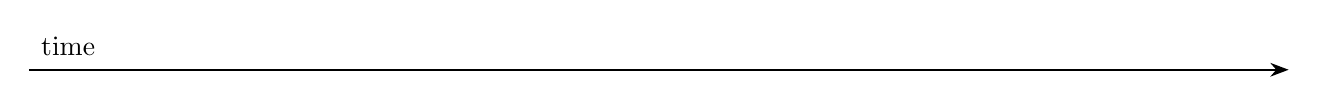
\begin{tikzpicture}
            % Zeit "Time" über dem Pfeil links positionieren
            \node at (-7.5, 0.3) {time}; % Text "Time"
            \draw[-Stealth, thick] (-8, 0) -- (8, 0); % Pfeil von ganz links nach ganz rechts
        \end{tikzpicture}
    \end{minipage}

    % Beschriftung unter dem Grid
    \vspace{0.5cm}
    \caption{Comparison between the original and the adapted auto-crop including frames 100, 700, 1000, 1600, and 1900 of the evaluation video \cite{temporalDataset_youtube_video}.
    The first row is the original auto-crop from \cite{tepNet2024} and the second row is the proposed one.}
    \label{fig:autocropVideoComparison}
\end{figure}

\begin{figure}[H]
    \centering
    \begin{subfigure}{\textwidth}
        \centering
        \includegraphics[width=\textwidth]{PICs/experiments/autocropExperiments/original_updated.jpg} % erstes Bild
        \caption{Original auto-crop mechanism}
        \label{fig:autocropResultsTrends_a}
    \end{subfigure}
    %\hspace*{0.02\textwidth} % Abstand manuell steuern
    \begin{subfigure}{\textwidth}
        \centering
        \includegraphics[width=\textwidth]{PICs/experiments/autocropExperiments/improved_updated.jpg} % zweites Bild
        \caption{Adapted auto-crop mechanism (Version 2)}
        \label{fig:autocropResultsTrends_b}
    \end{subfigure}
    \caption{Trend of the evaluation video \cite{temporalDataset_youtube_video} shown in \autoref{fig:autocropVideoComparison}.
    The first and third graphs with a single green line show the rail width at the first anchor line.
    The second and fourth graphs show crop coordinates (blue=left, red=right, green=top).
    Jumps in graphs from the adapted mechanism indicate resets, like the one at around frame 600.
    It also shows that with the original technique, cropcoords are stable and the prediction is not and the improved auto-crop reverses this relationship.}
    \label{fig:autocropResultsTrends}
\end{figure}


\noindent Models with a ResNet18 backbone show an additional behavior when uncertain.
The width of the predicted track becomes unstable, especially at the first few anchors.
This is because the camera is in a fixed position in this video \cite{temporalDataset_youtube_video}, and when correctly predicting the track, the width does not change at the bottom of the image.
Therefore, the track width at the first anchor line is a good indicator of uncertainty.
\autoref{fig:autocropVideoComparison} and \autoref{fig:autocropResultsTrends} show the evaluation of a model with the ResNet18 backbone on the evaluation video \cite{temporalDataset_youtube_video}.
\autoref{fig:autocropVideoComparison} shows the frames 100, 700, 1000, 1600, and 1900.
\autoref{fig:autocropResultsTrends} visualizes the trend of track width and crop coordinates.

As shown in frame 100, both models need time to find the right track.
The unstable rail width of both models also indicates this.
\autoref{fig:autocropResultsTrends_b} displays a jump of cropcoords and rail width at around frame 600, indicating a reset.
After that, the adapted auto-crop mechanism proves to be correct and stable.
However, in the video with the original cropping mechanism, the crop converges to an area that does not include the rail.
Since the system does not include a reset rule, it cannot recover from the mistake at the start.
When comparing both techniques in a broader scope, the original cropping mechanism shows stable crop coordinates, but the prediction is often incorrect.
On the other hand, the adapted technique moves more freely and quickly adapts to challenging scenarios.
Consequently, the prediction becomes more stable, which is the desired output.

\section{improved TEP-Net}
blindtext

\subsection{Backbones}
blindtext

\subsection{Pooling Layers}
blindtext

\subsection{Prediction Heads}
blindtext

\subsection{Sliding Window Approach}
blindtext

\subsection{Temporal Models}
blindtext

\section{Erste Überschrift Tiefe 2 (section)}
blindtext

\subsection{Erste Überschrift Tiefe 3 (subsection)}
blindtext

\subsubsection{Erste Überschrift Tiefe 4 (subsubsection)}
blindtext

%%%%%%%%%%%%%%%%%%%%%%%%%%%%%%%%%%%%%%%%%%%%%%%%%%%%%%%%%%%%%%%%%%
%%%%%%%%%%%%%%%%%%%%%%%%%%% Discussion %%%%%%%%%%%%%%%%%%%%%%%%%%%
\clearpage                                                       % Beginne neue Seite

% Include the first subsection from an external file
\chapter{Discussion}
\label{sec:discussion}

This chapter includes a discussion about gathered results.
Furthermore, the research questions introduced in the beginning of this work are addressed comprehensively and ultimately answered.
Therefore this chapter is devided into the individual research questions.

\subsubsection{1. What is the most effective vision-based approach for reliably identifying the rail track the train travels on, ensuring precise direction detection and robustness, especially in scenarios involving switches?}

\subsubsection{2. How can this application be implemented to run in real-time on an embedded device from the NVIDIA Jetson series?}

One goal of this work is to implement a real-time capable system.
All datasets in this work are some variations of RailSem19.
This dataset consists of images of YouTube videos primarily in 25 or 30 \ac{FPS}.
The temporal dataset also includes such videos.
Therefore, the system aims to speed up to 30 \ac{FPS}.
This results in a threshold for the latency of 33.33 ms or lower.
However, this is a simplified assumption based on available data rather than on a practical application.

When applied in an actual use case, the real-time capability primarily depends on the camera setup, the train velocity, the prediction, and the corresponding distances.
\autoref{fig:cameraSetup} shows a systematic camera setup with the most essential parameters, distances, and angles.
The green parts resemble the prediction with a length from the horizon line.

\autoref{func:RealTime} calculates the \ac{FPS} needed for a real-time capable system according to $d_{horizon}$ and $v_{train}$.
$d_{horizon}$ is defined by geometry of the camera setup.
Theoretically, the system is still fast enough when the train travels a distance of $d_{horizon}$ between each frame.
That corresponds to a $\lambda$ of 1.
Lamda is an additional parameter that defines how much the predicted area of the previous frame must overlap with the next frame.
Lambda must be between 0 and 1.
The lower the value, the safer the system becomes.

\begin{figure}[H]
    \centering
    \includegraphics[width=0.8\textwidth]{PICs/discussion/Kameraaufbau.pdf}
    \caption{Camerasetup}
    \label{fig:cameraSetup}
\end{figure}

\begin{align}
    FPS = \frac{v_{train}}{d_{horizon}} \times \frac{1}{\lambda}
    \label{func:RealTime}
\end{align}

\autoref{tab:variablesForRealTime} describes realistic values when the system is prepared for trains in Austria.
A GoPro Hero 10 \cite{goproHero10} is chosen because of its integrated mounting abilities and high $FoV$.
$\alpha$ and $height_{cam}$ are assumptions for Austrian trains.
$v_{train}$ is the fastest speed a train can drive in Austria \cite{geschwindigkeitZugAustria}.
Previous predictions like in \autoref{fig:autocropVideoComparison} lead to the assumption of $horizon_{pred}$.
480 pixels are roughly a third of the image that fits most predictions in this work.
\autoref{func:FPSValues} shows that only a speed of 5.1 \ac{FPS} is needed for a practical use case with the assumed parameters.
However, to increase safety, the overlap factor $\lambda$ is set to 0.17, which results in a frame rate of 30 \ac{FPS}.
Also interesting is that with this frame rate and the highest possible train speed, the distance traveled between frames is 2.45 m, as shown in \autoref{func:distanceBetweenFrameswith30FPS}.

\begin{table}[H]
    \centering
    \begin{tabular}{|l|c|c|}
    %\begin{tabular}{| p{0.3\linewidth} | p{0.6\linewidth} |}
        \hline
        \textbf{Parameters} & \textbf{Variables} & \textbf{Assumptions}\\
        \hline
        Camera model & & GoPro Hero 10 Black \cite{goproHero10} \\
        \hline
        Vertical Field of View & $FoV$ & $93^\circ$ \cite{goproHero10} \\
        \hline
        Camera mounting angle & $\alpha$ & $90^\circ$ \\
        \hline
        Camera mounting height & $height_{cam}$ & 4 m \\
        \hline
        Train speed & $v_{train}$ & 265 km/h \cite{geschwindigkeitZugAustria} $ \Leftrightarrow\ $ 73.61 m/s\\
        \hline
        Predicted horizon line & $ horizon_{pred} $ & 480 pixel from top \\
        \hline
        Overlap factor & $\lambda$ & 0.17 \\
        \hline
    \end{tabular}
    \caption{Variables for real time calculation}
    \label{tab:variablesForRealTime}
\end{table}

\begin{align}
    d_{horizon} = \tan \left( \left( \frac{image_{height} - horizon_{pred}}{image_{height}} \times FoV \right) + \alpha - \frac{FoV}{2} \right) \times height_{cam}
    \label{func:dHorizon}
\end{align}

\begin{align}
    d_{horizon} = \tan \left( \left( \frac{720 - 480}{720} \times 93 \right) + 90 - \frac{93}{2} \right) \times 4 = 14.42 \, {m}
    \label{func:dHorizonValues}
\end{align}

\begin{align}
    FPS = \frac{v_{train}}{d_{horizon}} \times \frac{1}{\lambda} = \frac{73.61}{14.42} \times \frac{1}{1} = 5.1
    \label{func:FPSValues}
\end{align}

\begin{align}
    FPS = \frac{v_{train}}{d_{horizon}} \times \frac{1}{\lambda} = \frac{73.61}{14.42} \times \frac{1}{0.17} = 30
    \label{func:FPSValuesOverlap}
\end{align}

\begin{align}
    d_{frames} = \frac{v_{train}}{FPS} = \frac{73.61}{30} = 2.45 \, {m}
    \label{func:distanceBetweenFrameswith30FPS}
\end{align}

\vspace{1cm}

\begin{figure}[H]
    \centering
    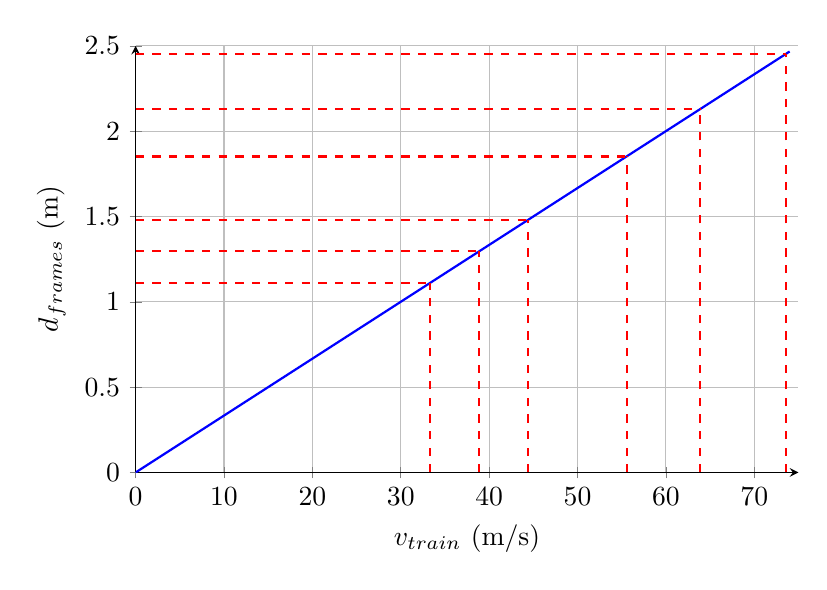
\begin{tikzpicture}
    \begin{axis}[
        width=10cm, height=7cm, % Größe des Graphen
        xlabel={$v_{train}$ (m/s)},
        ylabel={$d_{frames}$ (m)},
        xmin=0, xmax=75, % Begrenzung der x-Achse
        ymin=0, ymax=2.5, % Begrenzung der y-Achse
        grid=major,
        axis lines=left,
        legend style={at={(0.95,0.05)},anchor=south east},
        ]
        % Graph der Funktion y = 1/30 * x
        \addplot[blue, thick, domain=0:74, samples=100] {1/30 * x};
        
        % Vertikale und horizontale Linien für die gewünschten Geschwindigkeiten
        % 120 km/h = 33.33 m/s
        \draw[red, thick, dashed] (axis cs:33.33,0) -- (axis cs:33.33,1.111); % vertikal
        \draw[red, thick, dashed] (axis cs:0,1.111) -- (axis cs:33.33,1.111); % horizontal
        
        % 140 km/h = 38.89 m/s
        \draw[red, thick, dashed] (axis cs:38.89,0) -- (axis cs:38.89,1.2963); % vertikal
        \draw[red, thick, dashed] (axis cs:0,1.2963) -- (axis cs:38.89,1.2963); % horizontal
        
        % 160 km/h = 44.44 m/s
        \draw[red, thick, dashed] (axis cs:44.44,0) -- (axis cs:44.44,1.4813); % vertikal
        \draw[red, thick, dashed] (axis cs:0,1.4813) -- (axis cs:44.44,1.4813); % horizontal
        
        % 200 km/h = 55.56 m/s
        \draw[red, thick, dashed] (axis cs:55.56,0) -- (axis cs:55.56,1.8519); % vertikal
        \draw[red, thick, dashed] (axis cs:0,1.8519) -- (axis cs:55.56,1.8519); % horizontal
        
        % 230 km/h = 63.89 m/s
        \draw[red, thick, dashed] (axis cs:63.89,0) -- (axis cs:63.89,2.1297); % vertikal
        \draw[red, thick, dashed] (axis cs:0,2.1297) -- (axis cs:63.89,2.1297); % horizontal
        
        % 265 km/h = 73.61 m/s
        \draw[red, thick, dashed] (axis cs:73.61,0) -- (axis cs:73.61,2.4537); % vertikal
        \draw[red, thick, dashed] (axis cs:0,2.4537) -- (axis cs:73.61,2.4537); % horizontal
        
    \end{axis}
    \end{tikzpicture}
    \caption{Ratio between the train's speed and the distance it drives between frames with 30 \ac{FPS}. Red lines are top speeds of all different trains from Austria: 120 km/h, 140 km/h, 160 km/h, 200 km/h, 230 km/h, 265 km/h, \cite{geschwindigkeitAllTrainsAustria}}
    \label{fig:ratioSpeedDistanceBetweenFrames}
\end{figure}

Based on the calculated values required to assess a model's real-time capabilities, the following conclusions are drawn.
Tables in \autoref{improvedTEPNetResults} show that almost every single-frame-based model achieves latencies below the threshold of 33.33 ms which comes from a high frame rate of 30 \ac{FPS}.
This can be explained by the leight weight model architecture.
Only some versions of DenseNet exceed the desired target.

For answering this research question for the temporal models more factors must be considered.
\autoref{tab:temporalModelsResultsLatency} shows that the fastest temporal model is CNN\_FLAT\_FC in FP16.
Compared to the single-frame-based model, this method suffers from an increased latency, which is too high for inferring videos with 30 \ac{FPS}.
According to the calculations of \autoref{func:FPSValues}, the theoretical frame rate needed for real-time is 5.1 \ac{FPS}, which corresponds to a latency of 196.08 ms.
Since all temporal FP16 models have latencies below that, they are all theoretically real-time-capable.
FP32 models are too slow.

However, various methods could allow higher frame rates in practical operations.
Firstly, an increase in speed can be achieved by utilizing a MobileNet backbone.
\autoref{tab:temporalModelsResultsLatency} shows that this increases speed significantly and is within the limits of real-time capability when inferring 30 \ac{FPS} videos.
Secondly, only every third or fourth frame can be used, which reduces the frame rate and increases the allowed latency.
An additional advantage of only inputting every third or fourth frame into the model is that the temporal context window increases even when the length of the sliding window remains the same.
Even though information between frames is lost, ten frames would cover a window of 30 or 40 frames.
Furthermore, using this technique decreases the number of frames in which the train is located directly over the switch, resulting in a smaller time frame that needs to be bridged.

In conclusion, temporal models can operate in real-time with a frame rate of 5.1 \ac{FPS}.
However, this presents an extreme case with an overlap factor of 1, which decreases the possible safety of the system.
That leads to the thought that the optimal trade-off must be found between the overlap of the predicted areas of consecutive frames and the frame rate.
Furthermore, in a practical application also the train's current speed can be incorporated which changes the real-time threshold and therefore frame rate adaptively.

\subsubsection{3. To what extent can the temporal dimension be leveraged to improve the accuracy of predictions in switch situations where the necessary information is no longer present in the current frame?}

\autoref{tab:temporalModelsResults} shows scenarios exist in which the original auto-crop is more advantageous than the adapted one, even though \autoref{sec:autocropResults} and \autoref{sec:qualitativeComparison} prove that the adapted one is more robust.
After analyzing models in these test cases, it becomes evident that the higher accuracy in \textbf{Switch 2} and \textbf{Switch 4} highly depends on the specific situations of these sequences.
\textbf{Switch 2} is a very complex situation with many steep angled switches present in the sequence, which is unusual and only in train stations or shunting yards.
\textbf{Switch 4}, on the other hand, is easy and is similar to a simple straight rail in which a single-frame-based model performs with high accuracy, and there is no need for a temporal model.
In conclusion, the temporal component of the system is an approach to stabilize the single-frame-based model in switch scenarios.
However, when the scene is challenging, even the temporal models struggle, and when a scene is too easy, there is no need to try to stabilize the model.
The results of these two sequences lead to the thought that the created temporal dataset is not optimal and needs to be reviewed and changed.
In the fourth version of the dataset, questionable scenes like \textbf{Switch 2} and \textbf{Switch 4} can be removed.
Additionally, the sequence length can be increased, and other scenarios can be included, like ones for trams, which is not the case until now.

It must be mentioned that even though temporal models bring a performance gain at frames in which the train is located directly over a switch, single-frame-based models outperform temporal models in scenes without switches, according to the \ac{IoU}.
That is because single-frame-based models hit the rail pixels more precisely.

%%%%%%%%%%%%%%%%%%%%%%%%%%%%%%%%%%%%%%%%%%%%%%%%%%%%%%%%%%%%%%%%%%
%%%%%%%%%%%%%%%%%%%%% Conclusion and Outlook %%%%%%%%%%%%%%%%%%%%%
\clearpage                                                       % Beginne neue Seite

% Include the first subsection from an external file
\clearpage
\chapter{Conclusion and Outlook}
\label{sec:conclusionAndOutlook}

% Conclusion
From 2020 to 2023, rail traffic has significantly increased in Austria.
In these years, multiple switch-related accidents occurred, which resulted in fatalities.
An autonomous system can prevent such incidents when predicting the train's direction, particularly at switch cases.
However, state-of-the-art approaches often miss a key distinction between the train's rail track and others.

Therefore, this work aims to find the most effective vision-based approach for reliably identifying rail tracks.
This rail track prediction system distinguishes between rails currently used by the train and other rails visible in the image.
Additionally, this work primarily focuses on scenarios that include switches, which divide the rail track and the correct prediction of the train's path direction.
Furthermore, the pursuit of real-time capability emphasizes the importance of keeping the implemented models as lightweight as possible.

The state-of-the-art related to the rail domain includes only a few papers that make a difference between the train's rail track and others.
However, these introduce the concept of possible tracks, which include all possible paths a train could take.
When a switch is present in the scene, both paths are considered because of the assumption that the switch state cannot be determined correctly.

From this point, experiments are conducted with object detection models from the \ac{YOLO} series that focus on detecting and determining the state of upcoming switches.
The unsatisfactory results of these experiments led to the pursuit of a fundamentally different solution.

During these experiments with object detection models, a paper was published that introduces a promising approach by changing the problem formulation from a detection method to a regression technique.
This approach showed promising results and is therefore selected as a new baseline for further experiments of this work.
A significant portion of this work focuses on making this approach more robust.
Enhancements are achieved by experimenting with different backbones, model architectures, and cropping mechanisms that define the model's input.
Results on a tailored dataset that primarily focuses on unusual perspective angles and switch scenarios show that robustness can be improved.
The final optimized model demonstrates an improvement in accuracy of 6.61\% compared to the original model, with an increase in latency of less than 1 ms.
Despite this minor latency increase, the model remains well within the constraints of real-time performance thresholds.
Using a MobileNetV3-Backbone for this model still achieves an \ac{IoU} of 96.19\%, which is slightly below the original models (a maximal decrease of 1.34\%).
However, latencies are reduced to 2.05 ms, proving a significant increase in speed. 

However, the main limitation of this system lies in the approach being single-frame-based.
That presents an issue when driving over switches, and the start of the switch blades is no longer visible in the image.
At that point in time, the system cannot identify the correct rail as it lacks the information from previous frames.
Therefore, this work develops an approach that includes the temporal aspect of these situations.
Various models are experimented with, which incorporate \ac{RNN}s to learn sequential context.
A sequential dataset tailored to this particular problem is created.
It consists of sequences with 76 frames in which trains drive over switches.
The sequences are auto-labeled with the single-frame-based model and manually corrected whenever necessary.
Consequently, the data augmentation, dataloading logic, and evaluation process are adapted to support video input instead of single images.
Transfer learning and a sliding window approach are used to train various temporal models.
The results of these experiments show an improved accuracy at frames in which the train is directly located over the switch.
When considering the most relevant temporal test sequences, temporal models achieve an increase in \ac{IoU} of up to 16.43\%.
Proving that exploiting the temporal dimension provides an advantage and can increase robustness further.
However, more research must be conducted when employing the system for a real-world application.
Especially, since temporal models show latencies up to 328.86 ms.

In addition to accuracy evaluations, all models are optimized with the NVIDIAs TensorRT framework, and latencies are measured on an NVIDIA Jetson AGX Xavier.
This work discusses the real-time capabilities of all single-frame and temporal models, either proving that they are below a certain threshold of video inference or presenting further approaches to make models real-time operable.

\vspace{2cm}

%Outlook
\noindent Results of temporal experiments show an improvement in frames where the train is located directly over a switch.
However, further research steps can include reviewing and extending the temporal dataset.
The length of sequences can be increased, and other situations, like tram scenes, can be added.
Unnecessary scenes can be removed.
Furthermore, only every third or fourth frame can be used in training, which simultaneously expands the temporal context window, decreases the number of frames over a switch, and helps with the real-time capability of the system.

A fundamentally different approach could include a similar technique, but the model predicts four rails instead of regressing only two rails.
In scenes with switches, these annotations are the four rails of the switch, labeled with increasing numbers from left to right.
When no switch is present, only two rails are visible.
Both are annotated twice in this case.
An additional part of the model must then be developed to decide which two of the four rails are the ones of the train.
The idea is to outsource the decision of which rails are used to a classifier while keeping the regression part of the model as accurate as possible.
Furthermore, this approach allows a temporal module to be employed only for the classification problem, significantly reducing complexity.
Since this is a fundamentally different approach, a tailored dataset and a new model must be developed.
Additionally, the loss function must be adapted.


%%%%%%%%%%%%%%%%%%%%%%%%%%%%%%%%%%%%%%%%%%%%%%%%%%%%%%%%%%%%%%%%%% Hier beginnen die Verzeichnisse.
\clearpage                                                       % Beginne neue Seite

\printbib                                                        % Literaturverzeichnis LaTeX-Zitier-Standard
%\printbib{Literatur}                                             % Literaturverzeichnis FH-Zitier-Standard
\clearpage

\listoffigures                                                   % Abbildungsverzeichnis
\clearpage

\listoftables                                                    % Tabellenverzeichnis
\clearpage

\listoflistings                                                  % Quellcodeverzeichnis
\clearpage

\phantomsection
\addcontentsline{toc}{chapter}{\listacroname}
\chapter*{\listacroname}
\begin{acronym}[XXXXX]
    \acro{ABC}[ABC]{Alphabet}
    \acro{WWW}[WWW]{world wide web}
    \acro{ROFL}[ROFL]{Rolling on floor laughing}
    \acro{CV}[CV]{Computer Vision}
    \acro{RGB}[RGB]{Red Green Blue}
    \acro{RSDS}[RSDS]{Railroad Segmentation Dataset}
    \acro{IR}[IR]{Infrared}
    \acro{TEP}[TEP]{Train Ego Path}
    \acro{GT}[GT]{Ground Truth}
    \acro{FOV}[FOV]{Field Of View}
    \acro{CNN}[CNN]{Convolutional Neural Network}
    \acro{ICT}[ICT]{Institute for Computer Technology}
    \acro{TU}[TU]{Technical University Vienna}
    \acro{GPU}[GPU]{Graphics Processing Unit}
    \acro{IoU}[IoU]{Intersection Over Union}
    \acro{CPU}[CPU]{Central Processing Unit}
    \acro{TPU}[TPU]{Tensor Processing Unit}
    \acro{ONNX}[ONNX]{Open Neural Network Exchange}
    \acro{DLA}[DLA]{Deep Learning Accelerator}
    \acro{NVDLA}[NVDLA]{NVIDIA Deep Learning Accelerator}
    \acro{ROI}[ROI]{Region of Interest}
    \acro{RNN}[RNN]{Recurrent Neural Network}
    \acro{MACs}[MACs]{Multiply-Accumulate Operations}
    \acro{SOTA}[SOTA]{State Of The Art}
    \acro{YOLO}[YOLO]{You Only Look Once}
    \acro{RCNN}[RCNN]{Regions with CNN features}
    \acro{SSD}[SSD]{Single Shot MultiBox Detector}
    \acro{PGI}[PGI]{Programmable Gradient Information}
    \acro{GELAN}[GELAN]{Generalized Efficient Layer Aggregation Network}
    \acro{FPN}[FPN]{Feature Pyramid Networks}
    \acro{ILSVRC}[ILSVRC]{ImageNet Large Scale Visual Recognition Challenge}
    \acro{VGGNet}[VGGNet]{Visual Geometry Group Network}
    \acro{ASPP}[ASPP]{Atrous Spatial Pyramid Pooling}
    \acro{SPP}[SPP]{Spatial Pyramid Pooling}
    \acro{FPS}[FPS]{Frames Per Second}
    \acro{TPE-Net}[TPE-Net]{Track Point Extraction and Association Network}
    \acro{CGNet}[CGNet]{Context Grided Network}
    \acro{BiSeNet}[BiSeNet]{Bilateral Semantic segmentation Net}
    \acro{NAS}[NAS]{Network Architecture Search}
    \acro{RA}[RA]{Running Average}
    \acro{EMA}[EMA]{Exponential Moving Average}
    \acro{FC}[FC]{Fully Connected}
    \acro{ReLU}[ReLU]{Rectified Linear Unit}
\end{acronym}

%\phantomsection
%\addcontentsline{toc}{chapter}{\listacroname}
%\chapter*{\listacroname}
%\begin{acronym}[XXXXX]
%    \acro{ABC}[ABC]{Alphabet}
%    \acro{WWW}[WWW]{world wide web}
%    \acro{ROFL}[ROFL]{Rolling on floor laughing}
%    \acro{CV}[CV]{Computer Vision}
%\end{acronym}
%%%%%%%%%%%%%%%%%%%%%%%%%%%%%%%%%%%%%%%%%%%%%%%%%%%%%%%%%%%%%%%%%% Hier beginnt der Anhang.
\clearpage
\appendix
\chapter{Anhang A}
\clearpage
\chapter{Anhang B}
\end{document}
%%%%%%%%%%%%%%%%%%%%%%%%%%%%%%%%%%%%%%%%%%%%%%%%%%%%%%%%%%%%%%%%%% Ende des Inhalts